%%%%%%%%%%%%%%%%%%%%%%%%%%%%%%%%%%%%%%%%%%%%%%%%%%%%%%%%%%%%%%%%%%%%%%%%%%%%%%%%
% Template for USENIX papers.
%
% History:
%
% - TEMPLATE for Usenix papers, specifically to meet requirements of
%   USENIX '05. originally a template for producing IEEE-format
%   articles using LaTeX. written by Matthew Ward, CS Department,
%   Worcester Polytechnic Institute. adapted by David Beazley for his
%   excellent SWIG paper in Proceedings, Tcl 96. turned into a
%   smartass generic template by De Clarke, with thanks to both the
%   above pioneers. Use at your own risk. Complaints to /dev/null.
%   Make it two column with no page numbering, default is 10 point.
%
% - Munged by Fred Douglis <douglis@research.att.com> 10/97 to
%   separate the .sty file from the LaTeX source template, so that
%   people can more easily include the .sty file into an existing
%   document. Also changed to more closely follow the style guidelines
%   as represented by the Word sample file.
%
% - Note that since 2010, USENIX does not require endnotes. If you
%   want foot of page notes, don't include the endnotes package in the
%   usepackage command, below.
% - This version uses the latex2e styles, not the very ancient 2.09
%   stuff.
%
% - Updated July 2018: Text block size changed from 6.5" to 7"
%
% - Updated Dec 2018 for ATC'19:
%
%   * Revised text to pass HotCRP's auto-formatting check, with
%     hotcrp.settings.submission_form.body_font_size=10pt, and
%     hotcrp.settings.submission_form.line_height=12pt
%
%   * Switched from \endnote-s to \footnote-s to match Usenix's policy.
%
%   * \section* => \begin{abstract} ... \end{abstract}
%
%   * Make template self-contained in terms of bibtex entires, to allow
%     this file to be compiled. (And changing refs style to 'plain'.)
%
%   * Make template self-contained in terms of figures, to
%     allow this file to be compiled.
%
%   * Added packages for hyperref, embedding fonts, and improving
%     appearance.
%
%   * Removed outdated text.
%
%%%%%%%%%%%%%%%%%%%%%%%%%%%%%%%%%%%%%%%%%%%%%%%%%%%%%%%%%%%%%%%%%%%%%%%%%%%%%%%%

\documentclass[letterpaper,dvipsnames,twocolumn,10pt]{article}
\usepackage{usenix}

% to be able to draw some self-contained figs
\usepackage{nopageno}
\usepackage{tikz}
\usepackage{cite}[sort]
\usepackage{amsmath}
\usepackage[labelfont=bf]{caption}

% \usepackage{titlesec}
\usepackage[compact]{titlesec}
\usepackage{booktabs}
\usepackage{enumitem}
\usepackage{xspace}

% figures
\usepackage{subcaption}
\usepackage{float}
\usepackage{cleveref}
\usepackage{amssymb}
\usepackage{tcolorbox}
\usepackage{stfloats}
\usepackage[section]{placeins}

% Listings
\usepackage[scaled=0.85]{beramono}
\usepackage{listings}
\usepackage{hyperref}
\usepackage[dvipsnames]{xcolor}

\newfloat{lstfloat}{htbp}{lop}
\floatname{lstfloat}{Listing}
\def\lstfloatautorefname{Listing} % needed for hyperref/auroref

\makeatletter
\newcommand{\nospaceS}{\S\@gobble}
\makeatother
\Crefname{section}{\nospaceS}{\nospaceS}
\Crefname{figure}{Fig.}{Figs.}
\Crefname{table}{Tab.}{Tabs.}
\Crefname{listing}{Lst.}{Lsts.}
\crefalias{lstlisting}{listing}

\newcommand\code[1]{\lstinline$#1$}

\lstdefinelanguage{PythonDiff} {
 keywords={for, in},
 keywordstyle=\color{BrickRed}\bfseries,
 ndkeywords={transfer},
 ndkeywordstyle=\color{NavyBlue}\bfseries,
 basicstyle=\footnotesize\ttfamily,
 identifierstyle=\color{black},
 sensitive=false,
 comment=[l]{+},
 commentstyle=\color{ForestGreen}\ttfamily\bfseries,
 showstringspaces=false,
 string=[s]{\#}{\.},
 stringstyle=\color{gray}\ttfamily,
}

\lstdefinelanguage{Python} {
 keywords={class, def, return, instanceof, if},
 keywordstyle=\color{BrickRed}\bfseries,
 ndkeywords={DataFrameSplit, NdArraySplit, SplitType, CPU, GPU, @oa, @oa_alloc},
 ndkeywordstyle=\color{NavyBlue}\bfseries,
 basicstyle=\footnotesize\ttfamily,
 identifierstyle=\color{black},
 sensitive=false,
 comment=[l]{\#},
 commentstyle=\color{gray}\ttfamily\bfseries,
 showstringspaces=false,
 string=[s]{"}{"},
 stringstyle=\color{ForestGreen}\ttfamily,
}

\lstdefinelanguage{Rust} {
 keywords={fn, trait, struct, bool, u32, u64, u16, u8, usize},
 keywordstyle=\color{BrickRed}\bfseries,
 ndkeywords={QuACK, Quacker, ClientQuacker, Quack},
 ndkeywordstyle=\color{NavyBlue}\bfseries,
 basicstyle=\footnotesize\ttfamily,
 identifierstyle=\color{black},
 sensitive=false,
 comment=[l]{///},
 commentstyle=\color{gray}\ttfamily\bfseries,
 showstringspaces=false,
 string=[s]{"}{"},
 stringstyle=\color{ForestGreen}\ttfamily,
}

\lstset{language=Python}

\renewcommand{\topfraction}{0.95}
\renewcommand{\bottomfraction}{0.95}
\renewcommand{\textfraction}{0.05}
\renewcommand{\floatpagefraction}{0.95}

\newcommand{\Sys}{Packrat\xspace}
\newcommand{\sys}{packrat\xspace}

\usepackage{microtype}

%-------------------------------------------------------------------------------
\begin{document}
%-------------------------------------------------------------------------------

\newcommand{\keith}[1]{\textcolor{red}{{\sf (KW: #1)}}}
\newcommand{\thea}[1]{\textcolor{red}{{\sf (TR: #1)}}}
\newcommand{\gina}[1]{\textcolor{red}{\sf {(GY: #1)}}}
\newcommand{\michael}[1]{\textcolor{red}{\sf {(MW: #1)}}}

%don't want date printed
\date{}

% make title bold and 14 pt font (Latex default is non-bold, 16 pt)
\title{\Large \bf In-Network Retransmissions for Encrypted Transport Protocols}

%for single author (just remove % characters)
\author{
Anonymous
% \and
% {\rm Second Name}\\
% Stanford University
% copy the following lines to add more authors
% \and
% {\rm Name}\\
%Name Institution
} % end author

\maketitle

%-------------------------------------------------------------------------------
\begin{abstract}
%-------------------------------------------------------------------------------

This paper describes and evaluates new techniques for
network-originated retransmissions for end-to-end transport
connections, yielding performance benefits for encrypted transport
protocols in lossy settings.  We use set-reconciliation techniques
based on the Rateless IBLT to let the receiver efficiently acknowledge
encrypted packets to a network function, without modifying the sender
or the underlying wire format. With these tools, endpoints can receive
network-originated retransmissions appropriate for them, without an
additional layer of encapsulation, tunnel, or link-layer
retransmissions.

% Lossy network paths can significantly harm application performance. Existing
% approaches such as link-layer retransmissions and connection-splitting either
% cannot be tuned to the connections that share the link, or are otherwise
% infeasible without ossification or credentialing the proxy. In this paper, we
% show how in-network retransmissions via a sidekick connection can enable a
% variety of performance enhancements---higher throughput, lower latency, and
% lower link overheads---for a variety of \textit{encrypted} transport protocols
% in these settings. We utilize set reconciliation techniques based on the quACK
% to refer to encrypted packets, without involving the data sender, and leave the
% underlying protocol unchanged on the wire and opaque to the
% performance-enhancing proxy.

% These in-network retransmissions require an on-path proxy located near the
% data \textit{receiver}, and scalability becomes challenging when the more
% complex decoding and retransmission logic is shifted from the endpoint to the
% proxy. To address this issue, we present an alternate construction of the quACK
% using the IBLT data structure, improving the efficiency of encoding and
% decoding operations. Combined with the insight that the quACK sender is
% co-located at the endpoint with the application ACK sender, we can send
% significantly fewer and smaller quACKs overall, minimizing the extra load
% introduced by the sidekick connection to the network.

\end{abstract}

\section{Introduction}
\label{sec:sidekick:intro}

In the Internet's canonical model, transport is end-to-end and implemented only
in hosts. Traditionally, routers and other network components forwarded IP
datagrams without regard to their payloads or flow membership~\cite
{saltzer1984endtoend, clark1988darpa}; only hosts thought about connections,
reliable delivery, or flow-by-flow congestion control.

In practice, however, the best behavior for a transport protocol depends on the
particulars of the network path. An appropriate retransmission or
congestion-control scheme for a heavily-multiplexed wired network wouldn't be
ideal for paths that include a high-delay satellite link, Wi-Fi with bulk ACKs
and frequent reordering, or a cellular WWAN~\cite
{kuhn2021quic-over-sat,goyal2017abc}.

By the 1990s, many networks had broken from the canonical model by deploying
in-network TCP accelerators, also known as ``performance-enhancing proxies''
(PEPs)~\cite{rfc3135}. TCP PEPs can split an end-to-end connection into
multiple concatenated connections~\cite
{kapoor2005achieving,caini2006pepsal,davern2011httpep,farkas2012splittcp,hayes2019mmwave},
buffer and retransmit packets over a lossy link~\cite
{balakrishnan1995snoop,polese2017milliproxy}, virtualize congestion
control~\cite{cronkite2016vcc,he2016acdc,mihaly2012mobilePEP}, resegment the
byte stream, and enable forward error correction, explicit congestion
notification, or other segment-specific enhancements. Because TCP isn't
encrypted or authenticated, PEPs can achieve this transparently, without the
knowledge or cooperation of end hosts. Roughly 20--40\% of Internet paths cross
at least one TCP PEP~\cite{imc2011handley, edeline2019bottomup}.

While many flows benefit from PEPs, their use carries a cost: protocol
ossification~\cite{papastergiou2017deossifying, edeline2019bottomup}. When a
middlebox inserts itself in a connection and enforces its preconceptions about
the transport protocol, it can thwart the protocol's evolution, dropping
traffic that uses an upgraded version or new options. TCP PEPs have hindered or
complicated the deployment of many TCP improvements, such as ECN++, tcpcrypt,
TCP extended options, and multipath TCP~\cite
{mandalari2018ecnplusplus,imc2011handley,raiciu2012multipathtcp}.

In response to this ossification, and to an increased emphasis on privacy and
security, post-TCP transport protocols have been designed to be impervious to
meddling middleboxes, by encrypting and authenticating the transport header. We
refer to these newer transport protocols as ``secure'' transport protocols. The
most prevalent is QUIC~\cite{rfc9000}, found in billions of installed Web
browsers and millions of servers~\cite{zirngibl2021quicdeployment}; other secure
transport protocols are used in WebRTC/SRTP~\cite{rfc8834webrtc},
Zoom~\cite{zoom}, BitTorrent~\cite{bittorrent}, and
Mosh/SSP~\cite{winstein2012mosh}.

This encryption means that middleboxes can't interpose themselves on a
connection or understand the sequence numbers of packets in transit. This
prevents PEPs from providing assistance, reducing---in some situations---the
performance of secure transport protocols~\cite
{border2020quicsat-presentation,kuhn2021quic-over-sat,martin2022bbr-quic-sat,border2020evaluating,kosek2022quicpep}.
It's possible to co-design protocols and PEPs to preserve security and privacy
while permitting assistance from credentialed middleboxes~\cite
{ford2008logjam,sherry2015blindbox, dogar2012tapa,iyengar2009flow}, but
challenging to do so without tightly coupling these components, risking
ossification and fragility.

In this chapter, we propose a method for in-network assistance of secure transport
protocols that tries to resolve this tension. Our approach leaves the transport
protocol unchanged on the wire: an encrypted end-to-end connection between hosts,
opaque to middleboxes and free to evolve. No PEPs are credentialed to decrypt
the transport protocol's headers.

Instead, we propose a second protocol to be spoken on an adjacent connection
between an end host and a PEP. We call this the \emph{\bf Sidekick protocol},
and its contents are \emph{about} the packets of the underlying, or ``base,''
connection. Sidekick PEPs assist end hosts by reporting what they've observed
about the packets of the encrypted base connection, without coupling their
assistance to the details of the base protocol. End hosts use this information
to influence decisions about how and when to send or resend packets on the base
connection, approximating some of the performance benefits of traditional PEPs.
We first proposed a similar functional separation in \cite{yuan2022sidecar},
and presented a concrete realization of the idea and its nuanced
interactions with real transport protocols in \cite{yuan2024sidekick}.

One key technical challenge with this approach is how the Sidekick can
efficiently refer to ranges of packets in an encrypted base connection. These
packets appear random to the middlebox, and referring to a range of, e.g., 100
encrypted packets in the presence of loss and reordering is not as simple as
saying ``up to 100'' when there are cleartext sequence numbers. In \Cref
{sec:quack}, we presented and evaluated a mathematical tool called a \emph
{\bf quACK} that concisely represents a selective acknowledgment of randomly
encrypted packets. In this chapter, we leverage the power sum quACK,
based on the insight that we can model the problem as a system of power
sum polynomial equations if there is a practical bound on the maximum number of
``holes'' among the packets being ACKed.

A second challenge is how the end host should use information from a Sidekick
connection to obtain a performance benefit for its base connection. Since the
performance benefit comes from changing behavior at the end host rather than
the middlebox, transport protocols need to incorporate this information into
their existing algorithms for, e.g., loss detection and retransmission, which
have gotten increasingly complex over time. To explore this, we designed a
Sidekick protocol and integrated it into client implementations in three scenarios:
\begin{itemize}[noitemsep,topsep=2pt]
\item A low-latency audio stream over an Internet path that includes a Wi-Fi path segment
  (low latency with loss), followed by a WAN path segment (higher latency
  with low loss). Can the Sidekick PEP reduce the de-jitter buffer delay
  by triggering earlier retransmissions on loss?

\item An upload over the same path. Can a secure transport protocol like QUIC,
  aided by a Sidekick PEP at the point between these two path segments, match
  the throughput of TCP over a connection-splitting PEP?

\item A battery-powered receiver, downloading data from the Internet over Wi-Fi.
  If the Wi-Fi access point sends Sidekick quACKs on behalf of the receiver,
  can it reduce the number of times the receiver's radio needs to wake up
  to send an end-to-end ACK?
\end{itemize}

\smallskip

A third technical challenge is how knowledge about \emph{where}
loss occurs along a path should influence a congestion-control scheme.
The challenge in any such scheme is how to maximize the congestion window
while sharing the network fairly with competing flows.
We present a path-aware modification to the CUBIC congestion-control
algorithm~\cite{ha2008cubic}, which we call \mbox{\textbf{PACUBIC}},
that approximates the congestion-control behavior of a PEP-assisted split TCP
CUBIC connection while making its decisions entirely on the host.

\paragraph{Summary of results.}

We implemented the Sidekick protocol in a low-latency media client
based on the WebRTC standard, and an HTTP/3 client using the Cloudflare
implementation of QUIC~\cite{quiche} and the \texttt{libcurl}~\cite{libcurl}
implementation of HTTP/3. We evaluated the three scenarios in
real-world and emulation experiments.
In real-world experiments using an unmodified local Wi-Fi network to access our
nearest AWS datacenter, the Sidekick was able to trigger early retransmissions
to fill in gaps in the audio of a latency-sensitive audio stream, reducing the
receiver's de-jitter delay from 2.3~seconds to 204~ms---about a 91\% reduction
(\Cref{fig:real-world}). The Sidekick was also able to improve the speed of an
HTTP/3 (QUIC) upload by about 50\%.

In emulation experiments of the ``battery-powered receiver'' scenario,
the Sidekick PEP was able to reduce the need for the receiver to send ACKs
by sending proxy acknowledgments on its behalf---ACKs the sender used
to advance its flow-control and congestion-control windows. The
receiver only needed to wake up its radio to send occasional
end-to-end ACKs, which the sender used to discard data from its
buffer (\Cref{fig:ack-reduction}).

Also in an emulation experiment, we confirmed that PACUBIC's
performance approximates a split CUBIC connection (two TCP CUBIC
connections separated by a PEP), responding to loss events on the
different path segments similarly to how the individual CUBIC flows would
(\Cref{fig:loss-vs-tput}). The results indicate that the Sidekick protocol's gains
do not come at the
expense of congestion-control fairness relative to a split CUBIC connection.

\smallskip

The rest of this chapter discusses three motivating scenarios for the Sidekick
(\Cref{sec:sidekick:motivating}), describes the concrete Sidekick protocol we
built around power sum quACKs (\Cref{sec:sidekick:init,sec:sidekick:sender}) and
its implementation in two base protocols (\Cref{sec:sidekick:implementation}),
and then evaluates the protocol in real-world (\Cref{sec:sidekick:real-world})
and emulation experiments (\Cref{sec:sidekick:emulation}).

\section{Background}
\label{sec:background}

We provide a brief history of loss recovery mechanisms in the network to
motivate the need for lightweight, non-ossifying, in-network retransmissions
for encrypted transport protocols.

\paragraph{End-to-end loss recovery.}

% End-to-end loss recovery has traditionally served two purposes: facilitating
% retransmissions in reliable connections and adapting congestion control.
In end-to-end loss recovery,
congestion control algorithms were traditionally designed to treat all loss as an indicator of
congestion~\cite{rfc5681tcp,rfc2001tcp}.
% congestion~\cite{rfc8985,rfc9000,rfc5681tcp,rfc2001tcp,ha2008cubic,cardwell2024bbrv3-ietf120}.
% only react upon congestive loss~\cite{2019ccacensus}.

With modern wireless networks and higher bit-error rates, recent developments
such as the BBR congestion control
% (Bottleneck Bandwidth and Round-trip propagation time)
algorithm have de-prioritized packet loss as a congestion
signal~\cite{cardwell2017bbr}. This change enables higher throughput but has
raised concerns regarding TCP fairness~\cite
{ware2019modeling,philip2024prudentia}. In response, the performance of newer
versions of BBR has regressed in lossy environments, suggesting a lasting trend
in the treatment of loss as a congestion signal regardless of its source~\cite
{atc-submission}.

% regarding fairness among competing flows, suggesting that packet loss---whether
% due to congestion or non-congestive factors---remains closely associated with
% congestion dynamics and needs to be considered by
% CCAs~\cite{ware2019modeling,philip2024prudentia}.

\paragraph{Link-layer loss recovery.}

Loss recovery at the link layer~\cite{3gpp5gstandard,le2022link,ieee80211e} can
mitigate some of the dramatic reactions of CCAs by hiding random loss from
endpoints.
% The local RTT is much shorter than the end-to-end RTT such that
% sporadic losses can be repaired much faster (milliseconds or less).
% Local
% retransmissions also minimize overhead as they are confined to the lossy path
% segment itself.
% Note link-layer retransmissions are not applicable to higher
% latency settings such as satellite networks.
Applications and transport protocols are oblivious to this
functionality, and there is a tradeoff to this reliability~\cite{klingler2018impact,kliazovich2012arqproxy}.
Retransmitting more often increases the chance
of success but increases the time needed, and may also introduce
jitter and reordering~\cite{leung2007overview}.
Low-latency applications may prefer to transmit new data instead, but
retransmitting less often means more loss.
There is no ideal configuration for all connections that share the link.

% Detecting loss and retransmitting packets at the link layer has great benefits.
% The local RTT is much shorter than the end-to-end RTT, such that sporadic
% losses can typically be repaired much faster. Such local retransmissions also
% minimize overhead, as they are confined to the lossy path segment itself. Link
% layer loss recovery, e.g. at Wi-Fi or cellular links, can hide random loss from
% the endpoints such that the dramatic reaction of CCAs is avoided; applications
% and transport protocols are oblivious to this
% functionality~\cite{ratnamwtcp1998,ieee80211e,kliazovich2012arqproxy,wong1997linklayerrtx}.
% Retransmissions by link layers are a common source of jitter, and,
% depending on the behavior of the link's receiver, they may contribute to
% reordering in the network~\cite{perf2006linklayerrtx,leung2007overview}.

% There is a trade-off between reliability and the delay that local
% retransmissions produce. Trying longer (i.e., more often) increases the time
% needed and the chance of success. Rather than trying to retransmit (and delay)
% old data, some applications may prefer transmitting newer data instead; thus,
% ideally, applications should be in control of this trade-off, but they are not.
% Various ideas to improve the communication between applications and wireless
% link layers have been put forward~\cite{kwbdgrr-tsvwg-net-collab-rqmts-04}, but
% with little success~\cite{rfc9049}. The new Standard Communication with Network
% Elements (SCONE) Working Group in the IETF now defines such signaling for QUIC,
% and Explicit Congestion Notification (ECN) is such a signal---but these are in
% the direction of the network offering information (``throughput advice'') to
% endpoints, not vice versa~\cite{rfc3168,brw-scone-analysis-00}.
% This is not completely true: the DSCP offers a signal. E.g., RFC 8325 describes
% how the DSCP should be mapped onto 802.11 networks. but this is a coarse-grain,
% unreliable signal (the field may be zeroed on the path), and I don't know if  a
% certain DSCP choice translates into limiting the number of retransmits. All in
% all, I think it's best to avoid this complication and ignore this.

\paragraph{Transport-specific mechanisms.}

Some transport-layer proxies split a connection into two or more segments
and optimize the connection for each segment. In addition to
TCP connection splitters~\cite{rfc3135,honda2011still,hayes2019mmwave},
selective forwarding units (SFUs) are
used for media streams where low-latency is critical, so retransmissions occur
closer to the data receiver~\cite{rfc7667,andre2018comparative}.

% the "proxyimportance" ref may sound like it's just about mmWave but it
%  contains 4G measurements, finding proxy deployment

With Snoop~\cite{balakrishnan1995snoop}, it is clear
that complexities emerge in how the proxy interprets
and modifies plaintext sequence numbers on the wire, which also ossifies TCP.
This paper aims to explore how such a proxy can send helpful in-network
retransmissions to a variety of encrypted protocols while preserving
end-to-end semantics, without access to such information.


These types of approaches make unwarranted assumptions about
transport headers ossify the protocol~\cite{papastergiou2017deossifying}.
By making reliability guarantees to the endpoint, the connection-splitting
proxies also fate share with the connection.


% Another disadvantage is that these proxies fate share with th
% Any type of proxy assistance that cannot ultimately fall back to end-to-end
% mechanisms mandates that the proxy fate share with the connection.

% However, this requires
% credentialing the proxy and would not work for encrypted protocols or
% applications that don't pay to host a CDN.

\paragraph{Protocol-agnostic transport assistance.}

Forward error correction can be used in lossy environments, but this
introduces significant overheads as entire packet contents (and not just
sequence numbers) must be encoded during transmission~\cite
{rfc9265}. FEC also requires participation from both endpoints.

Mechanisms that encapsulate packets
% I like the Kramer MASQUE paper b/c it talks about applying MASQUE as a PEP
% The RFC is the introduction of MASQUE, but seems like some people cite the 
% original draft too.
offer potential for reliability without decrypting packet contents, but their
primary focus tends to be security. VPNs introduce a costly
encryption layer.
MASQUE tunnels protocols over HTTP/3, and if used for local retransmissions
has the potential for complex nested loss recovery and congestion control
interactions~\cite{rfc9298masque,schinazi-masque-proxy-05,kramer2021masquepep}.
It is intended to function per-application, and the best known implementation
from Apple functions like a VPN~\cite{icloud-private-relay}.
These proxies may also not be on-path, which harms performance.

% The MASQUE standards allow configurations with local retransmissions, e.g. when
% implementing a MASQUE tunnel with HTTP/2 over TCP, but the specifications
% present this as a disadvantage---which it is indeed, since MASQUE tunnels are
% not defined to be chosen per application, and some applications may not desire
% the added delay from local retransmits at all. Instead, the best known
% implementation, Apple Private Relay, functions like a VPN, carrying all traffic
% of a user through MASQUE tunnels. Another disadvantage of MASQUE configurations
% with local retransmissions is that TCP, or QUIC, as a tunnel protocol, is a
% full-fledged transport implementation, including additional functions such as
% congestion control (i.e., carrying QUIC over TCP or QUIC produces nested
% congestion control loops).

% advises against using HTTP/3 in
% ``reliable'' mode due to the potential for complex nested loss recovery and
% congestion control interactions.
% \thea{Can't find citations for this recommendation in RFC.}


% While this does not exist to our knowledge, what about a tunneling approach
% To generically enhance transport layer reliability, one approach involves
% encapsulating the transport protocol within a reliable transport protocol at a
% proxy. This method allows for protocol separation without requiring
% credentialed access to packet contents, effectively integrating aspects of
% link-layer retransmissions and transport-layer connection splitting.

The Sidekick proxy provides protocol-agnostic assistance by sending
``quACKs'' of encrypted packets to an endpoint, but cannot retransmit
packets itself~\cite{yuan2024sidekick}. This limits its usefulness
to when the loss is near the data \textit{sender}.
However, client traffic (which is near the lossy last-mile) is typically heavier
in the downlink direction. In this paper, we similarly leverage set
reconciliation in eACKs for referring to encrypted packets,
but to send network-originated retransmissions.

% \section{Motivating scenarios}
\label{sec:sidekick:motivating}

\begin{figure}[t]
	\centering
	\includegraphics[width=0.8\linewidth]{sidekick/figures/sc_protocol.pdf}
\caption{The proxy generates quACKs, in-network acknowledgments, based on
the encrypted packets it observes in the base protocol. It quACKs to an end
host, the data sender, which sends or resends packets on the base protocol as a result.
Although we only show one side of the connection, the Sidekick could assist
either end host of a bidirectional flow.
}
\label{fig:sidekick:overview}
\end{figure}


We focus on three scenarios where end hosts benefit from in-network assistance.
In each one, a proxy provides feedback in the form of a quACK to an end
host: the data sender (\Cref{fig:sidekick:overview}). Recall that a quACK is a
``cumulative ACK + selective ACK'' over encrypted packet identifiers. The data
sender uses this feedback to influence its behavior on the base connection,
without altering the wire format.

To be clear: the Sidekick protocol is not tied to a specific base protocol
nor to how the end hosts use the quACK information. The base protocol does not
need to be reliable, nor to have unique datagrams---we implemented and evaluated
the same Sidekick protocol and the same proxy behavior across the different
scenarios in this paper.

\subsection{Low-latency media retransmissions}
\label{sec:sidekick:motivating:media}

Consider a train passenger using on-board Wi-Fi to have a low-latency audio
conversation, using WebRTC/SRTP~\cite{rfc8834webrtc}, with a friend. The
end-to-end network path contains a low-latency, high-loss ``near'' path
segment (the Wi-Fi hop) followed by a high-latency, low-loss ``far'' path
segment (the cellular and wired path over the Internet). The friend probably
suffers from poor connection quality, experiencing drops in the audio stream or
high de-jitter buffer delays from waiting for retransmitted packets to be
played in order (\Cref{fig:sidekick:real-world:media} in the real world,
\Cref{fig:sidekick:main-results:media} in emulation).

In the Sidekick approach, a PEP on the Wi-Fi access point sends quACKs to
the media client on the passenger's laptop, assisting the base connection.
The passenger's media client uses quACKs to retransmit packets sooner than they
would have using negative acknowledgments (NACKs) from the friend. The
end result is similar to the effect of PEPs such as
Snoop~\cite{balakrishnan1995snoop} and Milliproxy~\cite{polese2017milliproxy}
that leverage TCP's cleartext sequence numbers to trigger early retransmission
on lossy wireless paths.

\subsection{Emulating split congestion control in an HTTP/3 file upload}
\label{sec:sidekick:motivating:http}

Consider the same train passenger as before but uploading a large file over the
Internet with a reliable transport protocol. If the protocol were TCP, the
train could deploy a split TCP PEP at the access point. The split connection
allows quick detection and retransmission of dropped packets on the lossy Wi-Fi
segment, while opening up the congestion window on the high-latency cellular
segment.

However, secure transport protocols like QUIC can't benefit from (nor be harmed
by) connection-splitting PEPs. Without a PEP, QUIC relies on end-to-end
mechanisms over the entire path to detect losses, recover from them, and adjust
the congestion-control behavior. This leads to reduced upload speeds
(\Cref{fig:sidekick:real-world:pep-emulation} in the real world,
\Cref{fig:sidekick:main-results:pep-emulation} in emulation).

With help from the same Sidekick PEP, the QUIC client combines information from
quACKs and end-to-end ACKs to emulate the congestion-control behavior of a
split TCP connection (\Cref{sec:sidekick:pacubic}). The
application considers whether packets are lost on the near or far path
segments, and adjusts the congestion window accordingly while respecting the
opacity of the end-to-end base connection. The application also retransmits the
packet as soon as the loss has been detected.

The only guarantee the proxy makes to the client via the quACK is that it has
received some packets. To respect the end-to-end reliability contract with the
server, the client does not delete packets that may need to be transmitted
until it receives an end-to-end ACK from the server, even if the packet has
been quACKed by the proxy.

\subsection{Battery-saving ACK reduction}
\label{sec:sidekick:motivating:ack-reduction}

Now consider a battery-powered device downloading a large file from the
Internet. To reduce how often the device's
radio needs to wake up, saving energy, the base connection can reduce the
frequency of end-to-end ACKs the device sends to the data sender.
ACK reduction has also been shown to improve performance by reducing collisions
and contention over half-duplex links~\cite{custura2023reducing,li2020tack}.
The ACK frequency can be configured with a TCP kernel setting or proposed
QUIC extension~\cite{ietf-quic-ack-frequency-07}.

However, ACK reduction can also degrade
throughput~\cite{custura2023reducing,custura2020impact}
(\Cref{fig:sidekick:main-results:ack-reduction} in emulation).
The data sender receives more delayed feedback about loss, and has to carefully
pace packets to avoid bursts in the large delay between ACKs.
One proposal has the PEP acknowledge packets on behalf of the data
receiver~\cite{kliazovich2012arqproxy}, leveraging cleartext TCP sequence
numbers. This proposal does not apply to secure transport protocols without
these sequence numbers.

In this scenario, a Sidekick proxy at a Wi-Fi access point or cellular base station
quACKs to the data sender on behalf of the battery-powered device. The device still occasionally
wakes up its radio to send ACKs, but the data sender uses the more frequent quACKs
from the proxy to advance its flow-control and congestion-control windows.

The data sender respects the end-to-end reliability contract by only deleting packets
in response to end-to-end ACKs, but disregards the data receiver's flow control by using quACKs
to advance the flow-control window. If the data sender only used end-to-end ACKs to advance the
window, it would waste time waiting between ACKs to send packets with too small
a window, and need to pace sent packets on receiving a large ACK with too large
a window.

\chapter{Sidekick Protocol}
\label{sec:sidekick}

In this paper, we propose a method for in-network assistance of opaque transport
protocols that tries to resolve this tension. Our approach leaves the transport
protocol unchanged on the wire: a secure end-to-end connection between hosts,
opaque to middleboxes and free to evolve. No PEPs are credentialed to decrypt
the transport protocol's headers.

Instead, we propose a second protocol to be spoken on an adjacent connection
between an end host and a PEP. We call this the \emph{\bf Sidekick protocol},
and its contents are \emph{about} the packets of the underlying, or ``base,''
connection. Sidekick PEPs assist end hosts by reporting what they've observed
about the packets of the opaque base connection, without coupling their
assistance to the details of the base protocol. End hosts use this information
to influence decisions about how and when to send or resend packets on the base
connection, approximating some of the performance benefits of traditional PEPs.
A similar functional separation was first proposed by \cite
{yuan2022sidecar}, but this paper presents the first concrete realization of
the idea and its nuanced interactions with real transport protocols.

One key technical challenge with this approach is how the Sidekick can
efficiently refer to ranges of packets in an opaque base connection. These
packets appear random to the middlebox, and referring to a range of, e.g., 100
opaque packets in the presence of loss and reordering is not as simple as
saying ``up to 100'' when there are cleartext sequence numbers. In \Cref
{sec:quack}, we present and evaluate a mathematical tool called a \emph
{\bf quACK} that concisely represents a selective acknowledgment of opaque,
randomly identified packets. The quACK is based on the insight that we can
model the problem as a system of power sum polynomial equations if there is a
practical bound on the maximum number of ``holes'' among the packets being
ACKed. We created an optimized implementation~\cite{quack-github}, building on
related theoretical work~\cite
{eppstein2011straggler,minsky2003set,karpovsky2003data}.

A second challenge is how the end host should use information from a Sidekick
connection to obtain a performance benefit for its base connection. Since the
performance benefit comes from changing behavior at the end host rather than
the middlebox, transport protocols need to incorporate this information into
their existing algorithms for, e.g., loss detection and retransmission, which
have gotten increasingly complex over time. To explore this, we designed a
Sidekick protocol we call Robin, and implemented it in three scenarios:
\begin{itemize}[noitemsep,topsep=2pt]
\item A low-latency audio stream over an Internet path that includes a Wi-Fi path segment
  (low latency with loss), followed by a WAN path segment (higher latency
  with low loss). Can the Sidekick PEP reduce the de-jitter buffer delay
  by triggering earlier retransmissions on loss?

\item An upload over the same path. Can an opaque transport protocol like QUIC,
  aided by a Sidekick PEP at the point between these two path segments, match
  the throughput of TCP over a connection-splitting PEP?

\item A battery-powered receiver, downloading data from the Internet over Wi-Fi.
  If the Wi-Fi access point sends Sidekick quACKs on behalf of the receiver,
  can it reduce the number of times the receiver's radio needs to wake up
  to send an end-to-end ACK?
\end{itemize}

\smallskip

A third technical challenge is how knowledge about \emph{where}
loss occurs along a path should influence a congestion-control scheme.
The challenge in any such scheme is how to maximize the congestion window
while sharing the network fairly with competing flows.
We present a path-aware modification to the CUBIC congestion-control
algorithm~\cite{ha2008cubic}, which we call \mbox{\textbf{PACUBIC}},
that approximates the congestion-control behavior of a PEP-assisted split TCP
CUBIC connection while making its decisions entirely on the host.

\paragraph{Summary of results.}

We implemented Robin in a low-latency media client
based on the WebRTC standard, and an HTTP/3 client using the Cloudflare
implementation of QUIC~\cite{quiche} and the \texttt{libcurl}~\cite{libcurl}
implementation of HTTP/3. We evaluated the three scenarios in
real-world and emulation experiments.
In real-world experiments using an unmodified local Wi-Fi network to access our
nearest AWS datacenter, the Sidekick was able to trigger early retransmissions
to fill in gaps in the audio of a latency-sensitive audio stream, reducing the
receiver's de-jitter delay from 2.3~seconds to 204~ms---about a 91\% reduction
(\Cref{fig:real-world}). The Sidekick was also able to improve the speed of an
HTTP/3 (QUIC) upload by about 50\%.

In emulation experiments of the ``battery-powered receiver'' scenario,
the Sidekick PEP was able to reduce the need for the receiver to send ACKs
by sending proxy acknowledgments on its behalf---ACKs the sender used
to advance its flow-control and congestion-control windows. The
receiver only needed to wake up its radio to send occasional
end-to-end ACKs, which the sender used to discard data from its
buffer (\Cref{fig:ack-reduction}).

Also in an emulation experiment, we confirmed that PACUBIC's
performance approximates a split CUBIC connection (two TCP CUBIC
connections separated by a PEP), responding to loss events on the
different path segments similarly to how the individual CUBIC flows would
(\Cref{fig:loss-vs-tput}). The results indicate that the Sidekick protocol's gains
do not come at the
expense of congestion-control fairness relative to a split CUBIC connection.

\smallskip

The rest of this paper describes the Sidekick's motivating scenarios
(\Cref{sec:sidekick:motivating}), discusses the concrete Sidekick protocol we
built around quACKs (\Cref{sec:sidekick:protocol}) and its implementation in two
base protocols (\Cref{sec:sidekick:implementation}), and then evaluates the
protocol in real-world and emulation experiments
(\Cref{sec:sidekick:evaluation}).

\section{Motivating applications}
\label{sec:sidekick:motivating}

\begin{figure}[t]
	\centering
	% \includegraphics[width=\linewidth]{figures/sc-legend.pdf}\\
	\includegraphics[width=\linewidth]{figures/sc_protocol.pdf}%
\caption{The proxy generates quACKs, in-network acknowledgments, based on
the opaque packets it observes in the base protocol. It quACKs to an end
host, the data sender, which sends or resends packets on the base protocol as a result.
Although we only show one side of the connection, the \sys could assist
either end host of a bidirectional flow.
\vspace{-0.4cm}
}
\label{fig:sc-protocols}
\end{figure}


We focus on three scenarios where end hosts benefit from in-network assistance.
In each one, a proxy server provides feedback, called a quACK, to an end host:
the data sender (\Cref{fig:sc-protocols}). Recall that a quACK is a
``cumulative ACK + selective ACK'' over encrypted sequence numbers. The data
sender uses this feedback to influence its behavior on the base connection,
without altering the wire format.

To be clear: the Sidekick protocol is not tied to a specific base protocol
nor to how the end hosts use the quACK information. The base protocol does not
need to be reliable, nor to have unique datagrams---we implemented and evaluated
the same Sidekick protocol and the same middlebox behavior across the different
scenarios in this paper.

\subsection{Low-latency media retransmissions}

Consider a train passenger using on-board Wi-Fi to have a low-latency audio
conversation, using WebRTC/SRTP~\cite{rfc8834webrtc}, with a friend. The
end-to-end network path contains a low-latency, high-loss ``near'' path
segment (the Wi-Fi hop) followed by a high-latency, low-loss ``far'' path
segment (the cellular and wired path over the Internet). The friend probably
suffers from poor connection quality, experiencing drops in the audio stream or
high de-jitter buffer delays from waiting for retransmitted packets to be
played in order (\Cref{fig:media} in emulation, \Cref
{fig:real-world:scenario1} in real world).

In the Sidekick approach, a Sidekick on the Wi-Fi access point sends quACKs to the audio
application on the user's laptop, assisting the base connection's data sender.
The sender uses quACKs to retransmit packets sooner than they would have using
negative acknowledgments (NACKs) from the receiver. The end result is similar
to the effect of prior PEPs, such as Snoop~\cite{balakrishnan1995snoop} and
Milliproxy~\cite{polese2017milliproxy}, that leverage TCP's cleartext sequence
numbers to trigger early retransmission on lossy wireless paths.

\subsection{Emulating split congestion control in an HTTP/3 file upload}

Consider the same train passenger as before but uploading a large file over the
Internet with a reliable transport protocol. If the protocol were TCP, the
train could deploy a split TCP PEP at the access point. The split connection
allows quick detection and retransmission of dropped packets on the lossy Wi-Fi
segment, while opening up the congestion window on the high-latency cellular
segment.

However, opaque transport protocols like QUIC can't benefit from (nor be harmed
by) connection-splitting PEPs. Without a PEP, QUIC relies on end-to-end
mechanisms over the entire path to detect losses, recover from them, and adjust
the congestion-control behavior. This leads to reduced upload speeds
(\Cref{fig:baseline-line} in emulation, \Cref{fig:real-world:scenario2} in real world).

With help from the same Sidekick PEP, the QUIC sender combines information from
quACKs and end-to-end ACKs to emulate the congestion-control behavior of a
split TCP connection (\Cref{sec:sidekick:protocol:sender-behavior}). The
application considers whether packets are lost on the near or far path
segments, and adjusts the congestion window accordingly while respecting the
opacity of the end-to-end base connection. The application also retransmits the
packet as soon as the loss has been detected.

The only guarantee the proxy makes to the sender via the quACK is that it has
received some packets. To respect the end-to-end reliability contract with the
receiver, the sender does not delete packets that may need to be transmitted
until it receives an ACK, even if the packet has been quACKed.

\subsection{Battery-saving ACK reduction}

Now consider a battery-powered device downloading a large file from the
Internet. To reduce how often the receiver's
radio needs to wake up, saving energy, the base connection can reduce the
frequency of end-to-end ACKs the device sends.
ACK reduction has also been shown to improve performance by reducing collisions
and contention over half-duplex links~\cite{custura2023reducing,li2020tack}.
The ACK frequency can be configured with a TCP kernel setting or proposed
QUIC extension~\cite{ietf-quic-ack-frequency-07}.

However, ACK reduction can also degrade throughput~\cite{custura2023reducing,custura2020impact}
(\Cref{fig:ack-reduction} in emulation).
The sender receives more delayed feedback about loss, and has to carefully
pace packets to avoid bursts in the large delay between ACKs.
One proposal has the PEP acknowledge packets on behalf of the
receiver~\cite{kliazovich2012arqproxy}, leveraging cleartext TCP sequence
numbers, but it does not apply to opaque transport protocols.

In this case, a Sidekick at the Wi-Fi access point (or a cellular base station)
quACKs to the sender on behalf of the receiver. The receiver still occasionally
wakes up its radio to send ACKs, but the sender uses the more frequent quACKs
to advance its flow-control and congestion-control windows.

The sender respects the end-to-end reliability contract by only deleting packets
in response to ACKs, but disregards the receiver's flow control by using quACKs
to advance the flow-control window. If the sender only used ACKs to advance the
window, it would waste time waiting between ACKs to send packets with too small
a window, and need to pace sent packets on receiving a large ACK with too large
a window.

\section{Sidekick Protocol design}
\label{sec:sidekick:protocol}

\paragraph{Configuration Messages.}

The data sender can send various other messages to the proxy
to configure the connection or reset bad state.

\paragraph{Resets.}
Robin allows the sender to tell the PEP to reinitialize the quACK.
This is helpful if the quACK becomes
invalid, e.g., if $m$ exceeds the threshold $t$. It is
always safe to reset the quACK, or even to ignore the Sidekick entirely and
fall back to the base protocol's end-to-end mechanisms.

\subsection{PEP discovery}
\label{sec:sidekick:protocol:discovery}

\newtcolorbox{protopayload}[2][]{
  colback=yellow!20,
  colframe=black,
  boxrule=0.5pt,
  arc=1pt,
  fontupper=\ttfamily,
  width=\linewidth,
  fonttitle=\small\bfseries,
  top=-1.5mm,
  bottom=-1.5mm,
  left=2mm,
  right=2mm,
  title={#2},
  #1
}

\begin{figure}[t]
    % \centering
    % Client payloads
    \begin{subfigure}[b]{0.48\linewidth}
        \begin{protopayload}{\texttt{Init}}
            \begin{lstlisting}[language=Rust,basicstyle=\footnotesize]
epoch: u32;
base_conn: [u8; 12];
eack_ty: u8;
num_symbols: u8;
id_offset: u16;
mem_bytes: u32;
            \end{lstlisting}
        \end{protopayload}
        \begin{protopayload}{\texttt{quACK}}
            \begin{lstlisting}[language=Rust,basicstyle=\footnotesize]
count: u32;
last_identifier: u32;
code: Vec<Symbol>;
            \end{lstlisting}
        \end{protopayload}
        \caption{Client payloads.}
        \label{fig:payloads:client}
    \end{subfigure}
    \hfill
    % Proxy payloads
    \begin{subfigure}[b]{0.48\linewidth}
        \begin{protopayload}{\texttt{InitACK}}
            \begin{lstlisting}[language=Rust,basicstyle=\footnotesize]
epoch: u32;
udp_port: u16;
errno: u32;
            \end{lstlisting}
        \end{protopayload}
        \begin{protopayload}{\texttt{Reset}}
            \begin{lstlisting}[language=Rust,basicstyle=\footnotesize]
epoch: u32;
errno: u32;
            \end{lstlisting}
        \end{protopayload}
        \begin{protopayload}{\texttt{Retransmit}}
            \begin{lstlisting}[language=Rust,basicstyle=\footnotesize]
udp_payload: Vec<u8>;
            \end{lstlisting}
        \end{protopayload}
        \caption{Proxy payloads.}
        \label{fig:payloads:proxy}
    \end{subfigure}
  % Caption
  \caption{Packrat protocol messages to initialize the connection and generate
   retransmissions. There are two constructions of the quACK: power sum and
   IBLT (\Cref{sec:quack}). The \texttt{Symbol} uses 5 and 4 bytes in each
   type, respectively.}
  \label{fig:payloads}
\end{figure}


Now we describe the messages that are exchanged in the
Packrat protocol (\Cref{fig:payloads}), starting with the handshake.

Our current design has senders signal quACK support by sending a
distinguished packet containing a 128-byte \emph{Sidekick-request} marker.  Such
inline signaling could confuse receivers, but Sidekicks target
protocols such as QUIC that discard cryptographically unauthenticated
data anyway.  It would be cleaner to signal support through
out-of-band UDP options~\cite{ietf-tsvwg-udp-options-28}, which we hope to do
once they are standardized.

The proxy replies to a Sidekick-request packet by sending a special packet
from the receiver's IP address and port number back to the sender.
This packet contains a \emph{Sidekick-reply} marker, an opaque session ID, and an
IP address and port number for communicating with the proxy.

Packrats are distinguished from other types of proxies such as VPNs and
transparent PEPs in that the proxy is on the path and the client is knowingly
receiving in-network retransmissions. In order to discover Packrat proxies on the
path, the client sends a magic discovery packet along the base connection
4-tuple, after it has established that connection. Proxies respond by
announcing that they support Packrat and their supported configurations, and the
server discards the invalid magic packet. Clients can choose to accept
assistance from a proxy by replying with an \texttt{Init} and their
configuration request. The proxy completes the handshake with an \texttt
{InitACK} and a new UDP address specific to this base connection.

\subsubsection{Explicit Proxy Configuration}

Sidekick connections can be configured explicitly or implicitly.  In systems that
explicitly configure proxies, such as Apple's iCloud Private Relay~\cite{icloud-private-relay}
based on MASQUE~\cite{kosek2021masque,kramer2021masquepep}, proxies can simply negotiate
sending quACKs during session establishment.  In most other settings,
such as 4G/5G cellular networks, PEPs have traditionally been deployed
as transparent proxies, silently interposing on end-to-end
connections.  Senders therefore need a way to detect transparent Sidekick
proxies and inform them of where to send quACKs.  Because of network
address translation, all communication to the proxy must be initiated
by the sender or use the same IP addresses and port numbers of the
base connection.

\subsubsection{Security}
A malicious third-party could execute a reflection amplification attack that
generates a large amount of traffic while hiding its source. This is
possible because the sender requests quACKs to a different port and (for some
carrier-grade NATs) IP address from the underlying session. To mitigate this,
each quACK contains a quota, initially 1, of remaining quACKs the proxy will
send as well as an updated session ID\@.
The quota and session ID ensure only the sender can increase the quota or
otherwise reconfigure the session.

An adversarial PEP could send misleading information to the sender. Note that
only on-path PEPs can send credible information, since they refer to unique
packet identifiers.
To mitigate this, the sender can consider PEP feedback along with
end-to-end metrics to determine whether to keep using the PEP. The sender can
always opt out of the PEP, and the PEP cannot actively manipulate traffic any
more than outside a Sidekick setting.

\subsection{Handshake}
\label{sec:sidekick:protocol:handshake}

Upon receiving the Sidekick-reply packet, the sender begins communicating
directly with the proxy from a different UDP port.  It initially sends
back the session ID and configuration parameters to start receiving
quACKs.

\paragraph{Protocol parameters.}
The sender configures (i) the quACK interval of the PEP and (ii) the threshold
number of missing packets $t$, or otherwise selects Sidekick-specific settings
such as how an identifier is computed.

The quACK interval is expressed in terms of time or number of packets,
 e.g., every $N$ milliseconds or every $N$ packets, as in a TCP delayed ACK.
The sender determines the desired interval based on its estimated
RTT of the base connection and its application objectives, e.g.,
more frequently for latency-sensitive applications or lower-RTT paths.

The threshold represents the bound on the number of missing packets
between quACKs, in practice the number of ``holes'' among the packets that are
selectively ACKed. The threshold depends on the quACK interval, and
should be set based on how precise loss detection needs to be and
other qualities of the link.
For example, the threshold is larger to detect congestive loss in the queue of a
bottleneck link, or smaller to still detect transmission error on a lossy link.

The proxy accepts or rejects these configurations with an \texttt{InitACK}, and
is ready to cache packets and retransmit. On receiving an \texttt{InitACK}, the
client is free to send quACKs.

\subsection{Proxy behavior: Send quACKs}
\label{sec:sidekick:protocol:proxy-behavior}

\subsection{Data sender behavior: Receive quACKs, retransmit packets, and path-aware congestion control}
\label{sec:sidekick:protocol:sender-behavior}

In this section, we discuss two particular sender-side behaviors that are enabled by
the Sidekick protocol and which are helpful across several scenarios: detecting packet loss
from a decoded quACK and congestion control.

\subsubsection{Detecting Loss}

The sender knows definitively which packets have been received by the proxy from
a decoded quACK. Next, it must determine from the remaining packets which ones
have been dropped and which are still in-flight, including if there has been a
reordering of packets. In-flight packets are later
classified as received or dropped based on future quACKs.

When there is no reordering, the packets that are dropped are just the ``holes''
among the packets that are selectively ACKed by the quACK. In particular, these
are the holes when considering sent packets in the order they were sent up to
the last element received, which represents the last selective ACK.
To identify these dropped packets, the sender encodes $t$ cumulative power sums
of its sent packets up to the last element received.
The difference between these power sums and the power
sums in the quACK represents the dropped packets. The sender ``removes'' the
identifiers of dropped packets from its cumulative power sums, ensuring that
the only packets that contribute to the threshold limit are those that
went missing since decoding the last quACK.
%  \michael{can we, instead of ``accumulates'', say: ``locally calculates'' ? This would seem clearer. Or are you trying to
% say that this is a continuously updated number?  If so, perhaps: ``locally calculates a cumulatively updated power sum quACK ...''?}

To account for reordering in loss detection, Robin implements an algorithm
similar to the 3-duplicate ACK rule in TCP~\cite{rfc5681tcp,rfc2001tcp}.
In TCP, if three or more duplicate ACKs are received in a row, it is a strong
indication that a segment has been lost. Robin considers a packet lost only if
three or more packets sent after the missing packet have been received.
Other mechanisms could involve timeouts for individual packets similar to the
RACK-TLP loss detection algorithm for TCP~\cite{rfc8985}.

\subsubsection{Path-Aware CUBIC Congestion Control}

Congestion-controlled base protocols must have a congestion response to lost
packets that they retransmit due to quACKs, similar to if the loss were
discovered by the end-to-end ACK.
This ensures friendliness with end-to-end congestion control algorithms that do
consider the loss, such as CUBIC~\cite{ha2008cubic} in the presence of a
connection-splitting TCP PEP.
Here, we propose PACUBIC, an algorithm that emulates this ``split CUBIC''
behavior. PACUBIC uses knowledge of where loss occurs to improve connection
throughput compared to end-to-end CUBIC, while remaining fair to competing flows.

Recall that CUBIC~\cite{ha2008cubic} reduces its congestion window by a
multiplicative decrease factor,
$\beta = \beta^* = 0.7$, when observing loss (a congestion event), and otherwise increases
its window based on a real-time dependent cubic function with scaling factor
$C=C^*=0.4$:
\[
cwnd = C(T-K)^3 + w_{max} \text{ where } K = \sqrt[3]{\frac{w_{max}(1-\beta)}{C}}.
\]

\noindent Here, $cwnd$ is the current congestion window,
$w_{max}$ is the window size just before the last reduction,
and $T$ is the time elapsed since the last window reduction.

While a split CUBIC connection has \emph{two} congestion windows,
end-to-end PACUBIC only has \emph{one} window representing the in-flight bytes
of the end-to-end connection.
Conceptually, we want an algorithm that enables PACUBIC's single
congestion window to match the sum of the split connection's two congestion
windows.

PACUBIC effectively makes it so that we reduce and grow $cwnd$
proportionally to the number of in-flight bytes on the path segment
of where the last congestion event occurred.
Let $r$ be the estimated ratio of the RTT of the near path segment
(between the data sender and the proxy) to the RTT of the entire connection
(between end hosts).
We use $r$ as a proxy for the ratio of the number of in-flight bytes.
If the last congestion event came from a quACK, we use the same real-time
dependent cubic function but with the following
constants\footnote{See \Cref{sec:appendix:pacubic} for more intuition behind $\beta'$ and $C'$.}
\[
\beta = 1 - r(1-\beta^*)\text{ and }C = \frac{C^*}{r^3}.
\]
\noindent If the last congestion event came from an end-to-end ACK, then we use
the original $\beta$ and $C$ as above.

While this algorithm resembles the congestion behavior of split CUBIC, it is
simply an approximation. PACUBIC does not know the exact number of bytes
in-flight on each path segment, and the sum of the two congestion windows is simply a
heuristic for an inherently different split connection. The main takeaway is
that knowing where loss occurs can inform congestion control. We generally
hope that quACKs can lead to the development of smarter, path-aware algorithms.

\section{Implementation}
\label{sec:sidekick:implementation}

\begin{table}[ht]
  \centering
  \begin{tabular}{l r r}
    \hline
    \textbf{Module} & \textbf{Language} & \textbf{LOC} \\
    \hline
    QuACK library (\Cref{sec:quack:microbenchmarks}) & Rust & 1772 \\
    Media server/client + integration & Rust & 478 \\
    \texttt{quiche} client integration & Rust & 1821 \\
    \texttt{libcurl} client integration & C & 1459 \\
    Proxy Sidekick binary & Rust & 833 \\
    \hline
  \end{tabular}
  \caption{Lines of code.
  }
  \label{tab:lines-of-code}
\end{table}


We now describe our implementation of Robin~\cite{sidekick-github} for several applications.
We integrated Sidekick functionality with a simple media client for low-latency streaming
and an HTTP/3 (QUIC) client.
The total implementation of the quACK library, and proxy and client
integrations used 6363 LOC (\Cref{tab:lines-of-code}).

\subsection{Applications}
\label{sec:sidekick:implementation:applications}

The baselines we evaluated against were the performance of two opaque transport
protocols without proxy assistance, and the fairness of a split CUBIC connection.

\paragraph{Low-latency media application.}
We implemented a simple server and client in Rust for streaming low-latency
media. The client sends a numbered packet containing 240 bytes of data every
20 milliseconds, representing an audio stream at 96 kbit/s.
The sequence number is encrypted on the wire.

The server receives packets. If it receives a nonconsecutive sequence number,
it sends a NACK back to the client that contains the sequence number of each
missing packet. The client's behavior on NACK is to retransmit the packet. The
server retransmits NACKs, up to one per RTT, until it has received the packet.

The server's application behavior is to store incoming packets in a buffer
and play them as soon as the next packet in the sequence is available. The
de-jitter buffer delay is the length of time between when the packet is stored
to when it can be played in-order. Some packets can be played immediately.

\paragraph{HTTP/3 file upload application.}
We used the popular \texttt{libcurl}~\cite{libcurl} file transfer library as the basis for
our HTTP client, and an \texttt{nginx} webserver. The client makes an HTTP
POST request to the server. Both are patched with \texttt{quiche}~\cite{quiche}, a production
implementation of the QUIC protocol from Cloudflare, to provide support for
HTTP/3.

For our TCP baselines, we used the same file upload application with the
default HTTP/1.1 server and client. We used a split-connection
TCP PEP~\cite{caini2006pepsal} that intercepts the TCP
SYN packet in the three-way handshake, pretends to be the other side of that
connection, and initiates a new connection to the real endpoint.
Both clients use CUBIC congestion control.

\subsection{Client integrations}
\label{sec:sidekick:implementation:client-integrations}

In each application, we modified only the \emph{client} to speak Robin
and respond to in-network feedback. The server remained unchanged.
The modifications were in two parts: following the discovery mechanism to
establish bi-directional communication with the proxy, and using the information
in the quACK to modify transport layer behavior.

\begin{table*}[h]
  \centering
  % \renewcommand{\arraystretch}{0.000023}
  \small
  \begin{tabular}{llllllll}
    \toprule
                 &                 &            & \bf QuACK     & \bf Thre-     &                                  & \bf Emu-   & \bf Real- \\
    \bf Scenario & \bf Link 1      & \bf Link 2 & \bf Interval & \bf shold     & \bf Success Metric               & \bf lated? & \bf World? \\
    \midrule
    \#1 Low-  & $1$ ms delay, $3.6\%$  & $25$ ms delay, $0\%$ & $2$ pkts & $8$ & Reduce tail latency of how long    & Yes & Yes \\
    latency           & loss, $100$ Mbit/s   & loss, $10$ Mbit/s    &         &      & packets are queued in the data     & & \\
    media &                      &                      &         &      & receiver's de-jitter buffer.   & & \\

    \#2 Connec-   & $1$ ms delay, $1.0\%$  & $25$ ms delay, $0\%$ & $30$ ms & $10$ & Achieve high throughput; match   & Yes & Yes \\
    tion- split-   & loss, $100$ Mbit/s   & loss, $10$ Mbit/s    &         &      & the performance, congestion con- & & \\
    ting PEP &                      &                      &         &      & trol behavior, and fairness of   & & \\
    emulation   &                      &                      &         &      & connection-splitting TCP PEPs.   & & \\

    \#3 ACK          & $25$ ms delay, $0\%$ & $1$ ms delay, $0\%$  & $15$ ms & $50$ & Reduce ACK frequency of data re- & Yes & No \\
    reduction    & loss, $10$ Mbit/s    & loss, $100$ Mbit/s   &         &      & ceiver; achieve high throughput. & & \\
    \bottomrule
  \end{tabular}
  \caption{Experimental scenarios. Link 1 connects the data sender (client) to
  the proxy, while Link 2 connects the proxy to the data receiver (server).
  The quACK interval and threshold represent our \sys configuration.
  \vspace{-0.3cm}
  }
  \label{tab:experimental-scenarios}
\end{table*}


\paragraph{Low-latency media client.} The media client has two open UDP sockets:
one for the base connection and one for the Sidekick connection. When it receives a
quACK, it detects lost packets without reordering and immediately retransmits
them. The protocol does not have a congestion window nor a flow-control window.
The client also sends reset and configuration messages over the Sidekick connection.

\paragraph{HTTP/3 file upload client.}
The HTTP/3 client similarly has an adjacent UDP socket for the Sidekick connection on
which it receives quACKs and sends reset and configuration messages. The client
passes the quACK to our modified \texttt{quiche} library, which interprets the
quACK and makes transport layer decisions. From the client's perspective,
\texttt{quiche} tells \texttt{libcurl} exactly what bytes to send over the wire.

Our modified \texttt{quiche} library uses the quACK to inform the
retransmission behavior, congestion window, and flow-control window. The library
immediately retransmits lost \emph{frames} in a newly-numbered
packet, as opposed to the lost \emph{packet}, similar to QUIC's original
retransmission mechanism. We implement PACUBIC,
described in \Cref{sec:sidekick:protocol:sender-behavior}.
We also move the flow-control window (without forgetting packets in the
retransmission buffer), but only in the ACK reduction scenario, when the
congestion window is nearly representative of that of the Sidekick connection's
path segment.

\subsection{Proxy}
\label{sec:sidekick:implementation:proxy}

Our proxy sniffs incoming packets of a network interface using the
\texttt{recvfrom} system call on a raw socket.
It stores a hash table using Rust's standard library \texttt{HashMap} that maps
socket pairs to their respective quACKs, and
incrementally updates the quACKs for flows that have requested Sidekick assistance.
It also sends quACKs at their configured frequencies and listens for
configuration messages.

\section{Evaluation methodology}
\label{sec:sidekick:evaluation:methodology}

We modeled the scenarios from \Cref{sec:sidekick:motivating}. We use the same
m4.xlarge AWS instance as before for the emulated experiments.

\subsubsection{Emulation}

We emulated a two-hop network topology (\Cref{fig:sc-protocols}) in mininet,
configuring the link properties using \texttt{tc}.
In emulation, we represented
each link by a constant delay (with variability induced by the queue), a random
loss percentage, and a maximum bandwidth.
\Cref{tab:experimental-scenarios} describes the parameters
for each link to model---e.g., lossy Wi-Fi or a high-latency cellular
path---as well as the metrics for success in that scenario.
Link 1 connects the data sender (client) to the proxy,
while Link 2 connects the proxy to the data receiver (server).
On the proxy, we either run a Sidekick,
a connection-splitting TCP PEP~\cite{caini2006pepsal}, or nothing at all.

\subsubsection{Real World}

To test its robustness, we also evaluated Robin over a real-world
environment that resembled the scenario on the train (\Cref{fig:setup:real}).
In this setup, a Lenovo ThinkPad laptop, running Ubuntu 22.04.3 with a 4-Core
Intel i7 CPU @ 2.60 GHz and 16 GB memory, acted as a client to an AWS instance in
the nearest geographical region. The ThinkPad used as an access point (AP)
a Lenovo Yoga laptop, running Ubuntu 20.04.6 with a 4-Core Intel i5 CPU @
1.60 GHz and 4 GB memory, with a 2.4 GHz Wi-Fi hotspot.
The AP was connected to the Internet via a JEXtream cellular modem
with a 5G data plan. The AP ran Sidekick software.

We measured the link properties of each path segment to compare to
our emulation parameters. We measured delay and loss using 1000~\texttt{ping}s
over a 100 second period, and bandwidth using an \texttt{iperf3} test.
On the near segment between the ThinkPad client and the AP,
the min/avg/max/stdev RTT was 1.249/37.194/272.168/54.660 ms
at 49.8 Mbit/s bandwidth. We observed that loss increased
the further away the AP. In our experiments, the client was located roughly
200 feet away in a different room, with 3.6\% loss.
The far segment between the AP and the AWS server was
48.546/64.381/92.374/6.806 ms with 0.0\% loss at 30.9 Mbit/s.
In both environments, the cellular link was the bottleneck link in terms of
bandwidth, and the corresponding path segments in emulation had similar
minimum RTTs and average loss percentages.

\section{Emulation results}
\label{sec:sidekick:evaluation}

\begin{figure}[t]
\centering
\includegraphics[width=\linewidth]{sidekick-paper/figures/setup_real.pdf}
\caption{Real-world experimental setup.
\vspace{-0.4cm}
}
\label{fig:setup:real}
\end{figure}

\begin{figure*}
% python latencies.py --percentile 99 --box-and-whiskers --http base quack_2p_8 -t 20
% python latencies.py --percentile 99 --box-and-whiskers -t 20
\begin{subfigure}{0.34\textwidth}
\includegraphics[width=\linewidth]{figures/fig4a_low_latency_media.pdf}
\caption{Scenario \#1: Low-latency media.
 Reduced tail latency of de-jitter delay
with earlier retransmission. 5 minute trials.}
\label{fig:media}
\end{subfigure}
\hfill
% python data_size_vs_tput.py --mean --median -t 10 --http quic quack_30ms_10 quack_60ms_20 quack_120ms_40
% python data_size_vs_tput.py --mean --median -t 10 --http quack_30ms_10 quic
\begin{subfigure}{0.31\textwidth}
\includegraphics[width=0.97\linewidth]{figures/fig4b_pep_emulation.pdf}
\caption{Scenario \#2: Connection-splitting PEP emulation. Improved goodput.
20 trials median. Error bars are 1st and 3rd quartiles.
}
\label{fig:baseline-line}
\end{subfigure}
\hfill
\begin{subfigure}{0.32\textwidth}
\includegraphics[width=0.99\linewidth]{figures/fig4c_ack_reduction.pdf}
\caption{Scenario \#3: ACK reduction.
High goodput independent of end-to-end ACK frequency.
10 MB upload.}
\label{fig:ack-reduction}
\end{subfigure}
\caption{
Comparing the end-to-end baseline protocol to the same protocol with a \sys
connection, using the success metrics for the three scenarios described in
\Cref{tab:experimental-scenarios}. The \textsf{\Sys($N$x)} data points show
the performance at $N$x the quACK interval (sent less frequently) and
threshold of the default configurations specified in
\Cref{tab:experimental-scenarios}.
\vspace{-0.3cm}
}
% \dm{Maybe a notation like $x/4$ would be more suggestive than $4x$?}
\label{fig:main-results}
\end{figure*}


We evaluated Robin to answer the following questions:
\begin{enumerate}[noitemsep,topsep=0pt]
	\item Can Sidekicks improve the performance of opaque transport protocols
	in a variety of scenarios while preserving the opaque behavior of the
	base protocols?
	\item Can a path-aware congestion control algorithm match the fairness of
	split TCP PEPs using CUBIC?
	\item How do the CPU overheads of encoding quACKs impact the maximum
	capacity of a proxy with a Sidekick?
	\item What link overheads does the power sum quACK add and how does it
	compare to the strawmen?
\end{enumerate}

\subsection{Performance of secure transport protocols with Sidekick}
\label{sec:sidekick:evaluation:main-results}

We first evaluate Robin's main performance goal: In each of the motivating
scenarios, we show that Robin can improve performance compared to the base
protocol alone, which would not be able to benefit from existing PEPs.
Each scenario has a different metric for success---tail latency, throughput,
or number of packets sent by the data receiver (corresponding to energy usage
or chance of Wi-Fi collisions)---demonstrating the versatility of the Sidekick
protocol.

\paragraph{Low-Latency Media.}
The Sidekick can reduce tail latencies in a low-latency media stream, representing
fewer drops and better quality of experience.
The early retransmissions induced by the Sidekick reduced the 99th percentile
latency of the de-jitter buffer delay from 48.6 ms to 2.2 ms---a 95\%
reduction (\Cref{fig:media}).
As long as the quACK interval is less than the end-to-end RTT, the connection
benefits from the Sidekick.

The Sidekick is beneficial in this scenario because it enables the client to sooner
detect and retransmit lost packets, and the server to sooner play packets from
its de-jitter buffer.
The end-to-end mechanism takes one additional received packet to notify of the
loss and
one end-to-end RTT to retransmit and play the packet (20+52=72ms), resulting in
three delayed packets (the three ``steps" in \Cref{fig:media}) in most cases.
The Sidekick takes up to two additional packets and one near path segment RTT
(20+2=22ms or 20$\times$2+2=42ms), delaying either one or two packets in comparison.
Dropped ACKs and quACKs account for the $<2\%$ of packets with even greater
de-jitter latencies.

\paragraph{Connection-Splitting PEP Emulation.}
The Sidekick improves upload speeds when there is a lossy, low-latency link
by using quACKs to inform the sender's congestion control.
In a scenario with $1\%$ random loss on the link between the proxy and the
data sender, the HTTP/3 (QUIC) client achieves $3.6\times$ the goodput for a 10 MB
upload with a Sidekick compared to end-to-end QUIC (\Cref{fig:baseline-line}).

When there is no random loss, the Sidekick does not impact the performance
of QUIC\@.
There are no logical changes to the base protocol in this case because all loss
is on the
bottleneck link on the far path segment, and the CPU overheads of processing quACKs
are negligible.

Knowing \emph{where} congestion occurs is an opportunity for creating smarter
congestion control. In PACUBIC, identifying where the loss occured let the data
sender reduce the congestion window proportionally to how many packets were
in-flight on each path segment. In \Cref{sec:sidekick:evaluation:pacubic}, we
will show that our path-aware congestion control algorithm still matches the
fairness of connection-splitting TCP PEPs.

\paragraph{ACK Reduction.}

Using quACKs in lieu of end-to-end ACKs allows the data receiver to
significantly reduce its ACK frequency while maintaining high goodput.
In our experiment, QUIC with a Sidekick sent $96\%$ fewer packets (mainly ACKs)
than end-to-end QUIC before the goodput dropped below 8.5 Mbit/s
(\Cref{fig:ack-reduction}).
The quACK enables the data sender to promptly move the flow-control window forward,
as long as the last hop is reliable.

The goodput significantly degrades when reducing the end-to-end ACK frequency
without a Sidekick. When end-to-end QUIC reduces the ACK frequency to every
80 ms, the data receiver sends $247 / 138 = 1.8\times$ the packets at
$4.5 / 8.4 = 0.5\times$ the goodput, worse than QUIC with the Sidekick
in both dimensions (\Cref{fig:ack-reduction}). With a Sidekick,
the data sender also does not need to change packet pacing to avoid bursts in
response to infrequent ACKs, which is why end-to-end QUIC cannot send fewer
than $\approx 240$ packets.

\subsubsection{Configuring the Sidekick Connection}
\Cref{tab:experimental-scenarios} shows the quACK interval and threshold we
elected for each scenario based on the considerations in
\Cref{sec:sidekick:protocol}. In each experiment in \Cref{fig:main-results},
we also show how with less frequent quACKs ($2\times$ and $4\times$ the
interval) and proportionally-adjusted thresholds, the protocol performs worse,
or more variably. Less frequent quACKs means the client reacts later to
feedback about the near path segment, and more often has to rely on the
end-to-end mechanism. The performance particularly degrades when the quACK
interval exceeds the end-to-end RTT. However, even in this case, the base
protocol with any Sidekick at all performs better than the base protocol alone\@.

\subsection{Link overheads from sending quACKs}
\label{sec:sidekick:evaluation:link-overheads}

\begin{figure}[h]
\begin{subfigure}{\columnwidth}
  % 5+
  %
  \setlength{\tabcolsep}{2pt}
  \footnotesize
  \centering
  \begin{tabular}{lccccccc}
    \toprule
    & \multicolumn{2}{c}{Data Sender$\rightarrow$} & \multicolumn{2}{c}{$\leftarrow$Proxy} & \multicolumn{2}{c}{$\leftarrow$Data Receiver} & \\
    & \bf Pkts & \bf Bytes & \bf Pkts & \bf Bytes & \bf Pkts & \bf Bytes & \bf Goodput \\
    \midrule
    QUIC E2E & $1.00\times$ & $1.00\times$ & $1.00\times$ & $1.00\times$ & $1.00\times$ & $1.00\times$ & $1.00\times$ \\
    Strawman 1a & $0.96\times$ & $1.01\times$ & \cellcolor{LighterRed}{$2.02\times$} & \cellcolor{LightestRed}{$1.56\times$} & $1.01\times$ & $1.03\times$ & \cellcolor{LighterGreen}{$3.33\times$} \\
    Strawman 1b & $0.94\times$ & $1.00\times$ & \cellcolor{LighterRed}{$2.00\times$} & \cellcolor{LightestRed}{$1.78\times$} & $1.00\times$ & $1.03\times$ & \cellcolor{LightGreen}{$3.53\times$} \\
    Strawman 1c & \cellcolor{LightestRed}{$1.83\times$} & $1.06\times$ & \cellcolor{LighterRed}{$2.01\times$} & \cellcolor{LightestRed}{$1.83\times$} & $1.00\times$ & $1.03\times$ & \cellcolor{LightGreen}{$3.46\times$} \\
    \bf \textcolor{black!50!blue}{Power Sum}   & \textcolor{black!50!blue}{\bf 0.94$\times$} & \textcolor{black!50!blue}{\bf 1.00$\times$} & \textcolor{black!50!blue}{\bf 1.03$\times$} & \textcolor{black!50!blue}{\bf 1.07$\times$} & \textcolor{black!50!blue}{\bf 1.00$\times$} & \textcolor{black!50!blue}{\bf 1.03$\times$} & \cellcolor{LightGreen}{\textcolor{black!50!blue}{\bf 3.55$\times$}} \\
    \bottomrule
  \end{tabular}
  % \includegraphics[width=\columnwidth]{figures/packet-overhead-retx.png}
  \caption{Scenario \#2: Connection-splitting PEP emulation.}
  \label{tab:packet-overhead:retx}
\end{subfigure}
\begin{subfigure}{\columnwidth}
  % \includegraphics[width=\columnwidth]{figures/packet-overhead-ackr.png}
  \setlength{\tabcolsep}{2pt}
  \footnotesize
  \centering
  \begin{tabular}{lccccccc}
    \toprule
    & \multicolumn{2}{c}{Data Sender$\rightarrow$} & \multicolumn{2}{c}{$\leftarrow$Proxy} & \multicolumn{2}{c}{$\leftarrow$Data Receiver} & \\
    & \bf Pkts & \bf Bytes & \bf Pkts & \bf Bytes & \bf Pkts & \bf Bytes & \bf Goodput \\
    \midrule
    QUIC E2E & $1.00\times$ & $1.00\times$ & $1.00\times$ & $1.00\times$ & $1.00\times$ & $1.00\times$ & $1.00\times$ \\
    Strawman 1a & $0.96\times$ & $1.00\times$ & \cellcolor{LightRed}{$9.94\times$} & \cellcolor{LighterRed}{$4.99\times$} & \cellcolor{LightGreen}{$0.04\times$} & \cellcolor{LightGreen}{$0.08\times$} & $1.02\times$ \\
    Strawman 1b & $0.96\times$ & $1.00\times$ & \cellcolor{LightRed}{$9.95\times$} & \cellcolor{LightRed}{$7.13\times$}      & \cellcolor{LightGreen}{$0.04\times$} & \cellcolor{LightGreen}{$0.08\times$} & $1.02\times$ \\
    Strawman 1c & \cellcolor{LightestRed}{$1.91\times$} & $1.05\times$ & \cellcolor{LightRed}{$9.73\times$} & \cellcolor{LightRed}{$7.41\times$}      & \cellcolor{LightGreen}{$0.04\times$} & \cellcolor{LightGreen}{$0.08\times$} & $0.97\times$ \\
    \bf \textcolor{black!50!blue}{Power Sum}    & \textcolor{black!50!blue}{\bf 0.96$\times$} & \textcolor{black!50!blue}{\bf 1.00$\times$} & \textcolor{black!50!blue}{\bf 1.09$\times$} & \cellcolor{LighterRed}{\textcolor{black!50!blue}{\bf 2.56$\times$}} & \cellcolor{LightGreen}{\textcolor{black!50!blue}{\bf 0.04$\times$}} & \cellcolor{LightGreen}{\textcolor{black!50!blue}{\bf 0.08$\times$}} & \textcolor{black!50!blue}{\bf 0.98$\times$} \\
    \bottomrule
  \end{tabular}
  \caption{Scenario \#3: ACK reduction.}
  \label{tab:packet-overhead:ackr}
\end{subfigure}
\caption{Link overheads for a 10 MB upload. The cells represent the multiplier
relative to the end-to-end QUIC baseline for each type of quACK\@.
Lower is better for number of packets and bytes sent on a link.
Higher goodput is better. Robin's power sum quACK achieves the success metric
for each scenario without incurring the link overheads of the strawmen.
We did not evaluate the contrived protocol in Scenario \#1.
}
\label{tab:packet-overhead}
\end{figure}


The other cost in terms of using Sidekick protocols is the additional data
sent by the proxy to the data sender.
Too many additional bytes use up bandwidth, and additional packets use
up CPU\@.
\Cref{tab:packet-overhead} shows the number of packets and bytes sent at each
node comparing the strawmen and power sum quACK to no Sidekick connection at all.

Using power sum quACKs increases the packets sent from the proxy to the data
sender
by 3-9\%. These packets either consist mostly
of end-to-end ACKs which are sent every packet in \texttt{quiche}, or end-to-end
ACKs that have been replaced by quACKs in the ACK reduction scenario.
We did not evaluate Scenario \#1 because it is based
on a contrived protocol that lacks many of these features, and the link
overheads would not really make sense.

This overhead is representative of the CPU overhead at the client, since
quACKs and ACKs take a similar number of cycles to process. In an experiment
with Scenario \#2 during a period of $\approx90$k incoming packets, ACKs took on
average 26065 cycles to process while the quACKs took 26369 cycles, 1\% more.
These cycles come from, i.e., the complex recovery and loss detection algorithms
implemented at the end host.

The strawmen have significantly higher link overheads compared to the power sum
quACK\@. The proxy sends up to 10$\times$ more packets using Strawman 1a, and
also slightly harms the goodput in the congestion control scenario.
The reduced goodput is due to the sender mis-identifying received packets as
dropped due to dropped quACKs.
The proxy achieves higher goodput with Strawman 1b but sends
more bytes. Strawman 1c increases the link overheads at both the proxy and the
data sender due to larger TCP headers and TCP ACKs.
We did not evaluate Strawman 2 due to its impractical decode time.

\subsection{CPU overheads of encoding at the proxy}
\label{sec:sidekick:evaluation:cpu-overheads}

\begin{table}[ht]
  \centering
  \small
  \begin{tabular}{lrrrr}
    \toprule
    & \multicolumn{2}{r}{\bf 25-Byte Payload} & \multicolumn{2}{r}{\bf 1468-Byte Payload}\\
    & \bf Cycles & \bf $\%$ & \bf Cycles & \bf $\%$ \\
    \midrule
    Sniff Packet & 22417 & 97.6 & 22408 & 97.5 \\
    Table Lookup &   247 &  1.1 &   251 &  1.1 \\
    Parse ID     &    23 &  0.1 &    22 &  0.1 \\
    Encode ID    &    74 &  0.3 &    69 &  0.3 \\
    Other        &   213 &  0.9 &   225 &  1.0 \\
    \midrule
    \emph{Total} & \emph{22974} & \emph{100.0} & \emph{22975} & \emph{100.0} \\
    \bottomrule
  \end{tabular}
  \caption{Breakdown of the CPU cycles spent processing each packet at the
  proxy. Most cycles are spent on general per-packet overheads as opposed to
  quACK-specific processing.
  }
  \label{tab:cpu-overhead}
\end{table}


The main bottleneck of Robin on a proxy is the CPU\@.
\Cref{tab:cpu-overhead} shows a breakdown of the number of CPU cycles in each
step. The largest overhead was reading the packet contents from the network
interface ($97.5\%$ of the CPU cycles).

Encoding an identifier in a power sum quACK with $t=10$ used $74$ CPU
cycles ($0.9\%$). As a calculation of the theoretical maximum on a 2.30 GHz
% 2.30e9 / 74 = 31 million
CPU, the proxy would be able to process $31$ million packets/second on a single
core. The hash table lookup used $251$ cycles and parsing the pseudorandom
payload as an identifier used $22$ cycles.

In practice, we measured the maximum throughput of Robin to
be 464k packets/s with 25-byte payloads and 5.5 Gbit/s (458k packets/s) with
1468-byte packet payloads on a single core (assuming 1500-byte MTUs).
This experiment used multiple \texttt{iperf3} clients to simulate high
load until Robin was unable to keep up with the load on a single core.
The packet payload size did not seem to affect results.

We find these achieved throughputs acceptable for edge routers such as Wi-Fi
APs and base stations.
To deploy Robin on core routers, we would need to reduce the overhead of reading
packets from the NIC, such as by bypassing the kernel/user-space
protection boundary\footnote{
A kernel-bypass system like Retina~\cite{wan2022retina} can achieve
25 Gbps on 2 cores while processing raw packets with a 1000-cycle callback
(Figure 5(a) in \cite{wan2022retina}). The Sidekick equivalent would be a 500-cycle
callback, and assuming all traffic has requested Sidekick help. Throughput scales
almost linearly with the number of cores using symmetric RSS hashing.
Thus we don't expect proxy overheads to be an issue with modern 100 Gbps network
speeds and an optimized implementation even on commodity hardware.
}~\cite{dpdk,mccanne1993bsd,wan2022retina}
or using native hardware~\cite{bosshart2014p4}.
We could also scale on multiple cores using symmetric RSS hashing~\cite{woo2012scalable}.

\subsection{TCP friendliness of path-aware CUBIC}
\label{sec:sidekick:evaluation:pacubic}

\begin{figure}[t]
\centering

\includegraphics[width=\columnwidth]{figures/fig5_baseline_bar_legend.pdf}
\begin{subfigure}{0.49\linewidth}
	\includegraphics[width=\linewidth]{figures/fig5_baseline_loss0p.pdf}
	\caption{0\% loss.}
	\label{fig:baseline-bar:loss0p}
\end{subfigure}
\begin{subfigure}{0.49\linewidth}
	\includegraphics[width=\linewidth]{figures/fig5_baseline_loss1p.pdf}
	\caption{1\% loss.}
	\label{fig:baseline-bar:loss1p}
\end{subfigure}
\vspace{-0.2cm}
\caption{Median goodput for three upload data sizes with $0\%$ and $1\%$ loss on
Link 1. 20 trials. Error bars are 1st and 3rd quartiles.
With proxy assistance at $1\%$
loss, both QUIC and TCP match the performance of when there is no loss at all.
\vspace{-0.4cm}
}
\label{fig:baseline-bar}
\end{figure}

\begin{figure}[t]
\centering

\includegraphics[width=\columnwidth]{figures/fig6_legend.pdf}
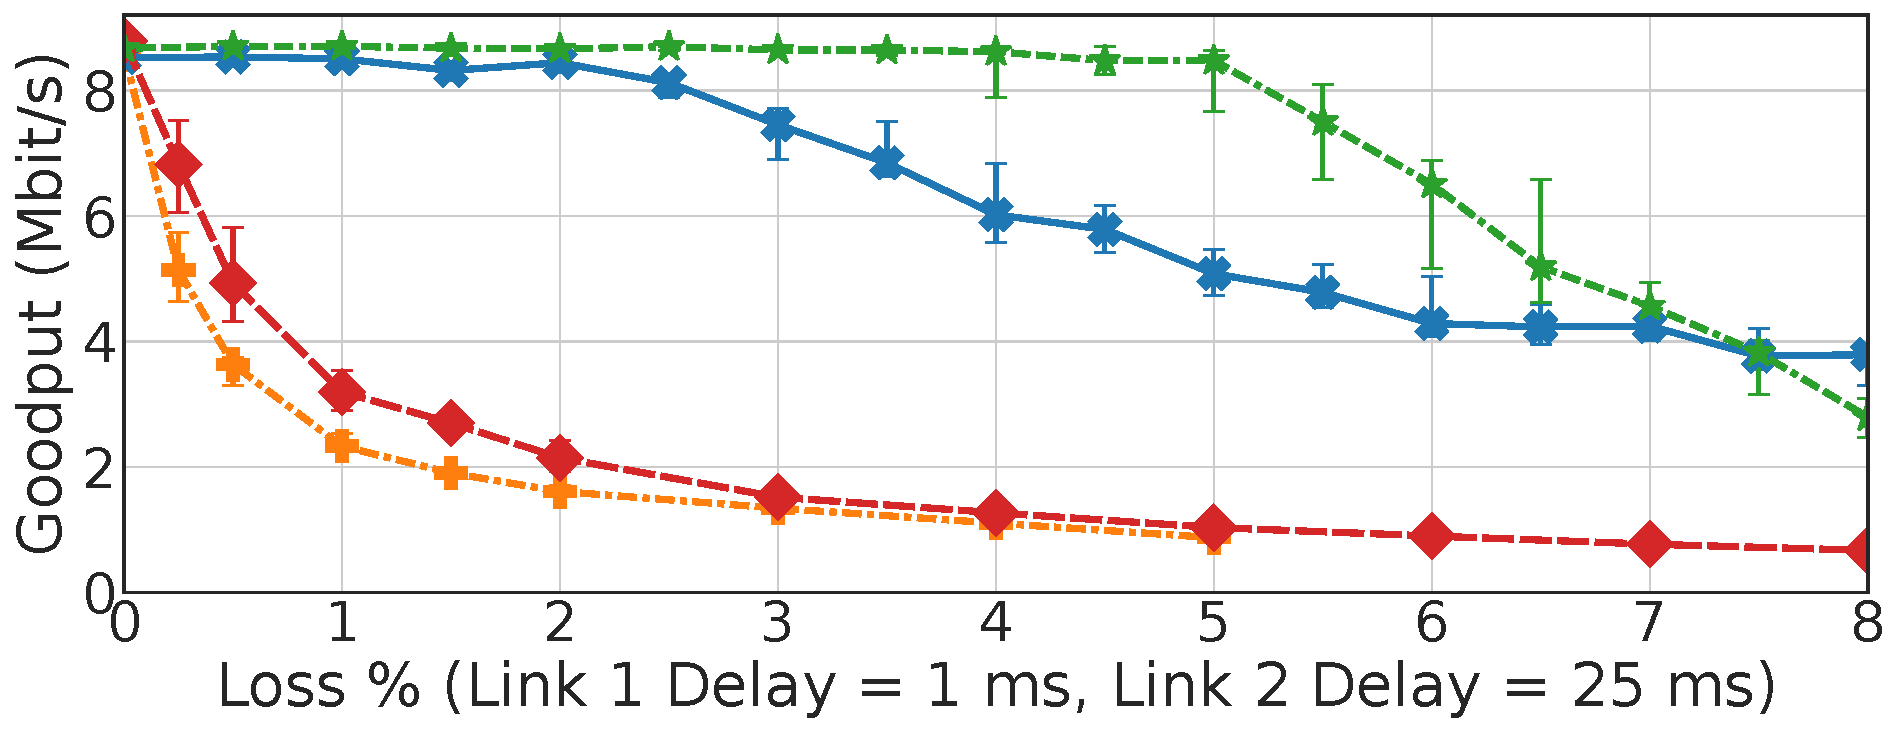
\includegraphics[width=\columnwidth]{figures/fig6_loss_bw100_10M_delay_25ms_1ms.pdf}
%\includegraphics[width=\columnwidth]{figures/loss_bw100_10M_delay_15ms_11ms.pdf}
\vspace{-0.4cm}
\caption{Connection-splitting PEP emulation as a function of near-segment
	loss rate. In this emulation experiment, QUIC+\Sys (running PACUBIC)
  performs similarly to TCP+PEP (each connection running CUBIC)
  and improves goodput compared with end-to-end protocols. The graph shows
  median goodput of a 10~MByte upload. QuACK interval is 30~ms, threshold
is 10. Error bars show IQR of 10 trials.
\vspace{-1cm}
}
\label{fig:loss-vs-tput}
\end{figure}

%\begin{figure}[t]
%\centering
%	\includegraphics[width=0.6\linewidth]{figures/multiflow_loss0p_legend.pdf}\\
%	\includegraphics[width=0.32\linewidth]{figures/quic_quack_60M_loss0p_delay0s_bw100.pdf}
%	\includegraphics[width=0.32\linewidth]{figures/quic_quack_60M_loss0p_delay5s_bw100.pdf}
%	\includegraphics[width=0.32\linewidth]{figures/quack_quic_60M_loss0p_delay5s_bw100.pdf}
%        \caption{Fairness evaluation of two concurrent QUIC flows in
%          Scenario \#1 (but without loss on the near path segment), one \sys-assisted and one end-to-end, in a purely
%          congestion-limited situation. The use of
%          \sys assistance doesn't affect 
%
%          Throughput of two concurrent flows in Scenario 1 (with $0\%$ and $1\%$
%loss on Link 1. Both flows converge to a steady-state throughput, whether the
%flows start at the same time (left) or at a 5 second delay (middle, right).}
%\label{fig:multiflow}
%\end{figure}

% \begin{figure*}
% \centering
% \includegraphics[width=\columnwidth]{figures/legend.pdf}\\
% \subfigure[QUIC, QUIC no delay]{
% 	\includegraphics[width=0.185\textwidth]{figures/quic_quic_60M_loss0p_delay0s.pdf}
% 	\label{fig:multiflow:a}}
% \subfigure[QUIC, QUIC 5s delay]{
% 	\includegraphics[width=0.185\textwidth]{figures/quic_quic_60M_loss0p_delay5s.pdf}
% 	\label{fig:multiflow:b}}
% \subfigure[QUIC, \sys no delay]{
% 	\includegraphics[width=0.185\textwidth]{figures/quic_quack_60M_loss0p_delay0s.pdf}
% 	\label{fig:multiflow:c}}
% % \subfigure[quack, quic no delay]{
% % 	\includegraphics[width=0.185\textwidth]{figures/quack_quic_60M_loss0p_delay0s.pdf}}
% \subfigure[QUIC, \sys 5s delay]{
% 	\includegraphics[width=0.185\textwidth]{figures/quic_quack_60M_loss0p_delay5s.pdf}
% 	\label{fig:multiflow:d}}
% \subfigure[\sys, QUIC 5s delay]{
% 	\includegraphics[width=0.185\textwidth]{figures/quack_quic_60M_loss0p_delay5s.pdf}
% 	\label{fig:multiflow:e}}
% % \label{fig:multiflow:quic-quack}
% % \end{figure*}

% % \begin{figure*}
% % \centering
% \subfigure[PEP, PEP no delay]{
% 	\includegraphics[width=0.185\textwidth]{figures/pep_pep_60M_loss1p_delay0s.pdf}
% 	\label{fig:multiflow:f}}
% \subfigure[PEP, PEP 5s delay]{
% 	\includegraphics[width=0.185\textwidth]{figures/pep_pep_60M_loss1p_delay5s.pdf}
% 	\label{fig:multiflow:g}}
% \subfigure[PEP, \sys no delay]{
% 	\includegraphics[width=0.185\textwidth]{figures/pep_quack_60M_loss1p_delay0s.pdf}
% 	\label{fig:multiflow:h}}
% % \subfigure[quack, pep no delay]{
% % 	\includegraphics[width=0.185\textwidth]{figures/quack_pep_60M_loss1p_delay0s.pdf}}
% \subfigure[PEP, \sys 5s delay]{
% 	\includegraphics[width=0.185\textwidth]{figures/pep_quack_60M_loss1p_delay5s.pdf}
% 	\label{fig:multiflow:i}}
% \subfigure[\sys, PEP 5s delay]{
% 	\includegraphics[width=0.185\textwidth]{figures/quack_pep_60M_loss1p_delay5s.pdf}
% 	\label{fig:multiflow:j}}
% \caption{Multiflow experiment with various combinations of QUIC end-to-end and QUIC+\sys at 0\% loss (a-e),
% and various combinations of TCP+PEP and QUIC+\sys at 1\% loss (f-j), demonstrating
% flow fairness. The delay indicates how long we started the second flow after the first flow.}
% \label{fig:multiflow}
% \end{figure*}


It is easy to improve performance without regard to competing flows;
however, we demonstrate that PACUBIC can
match the fairness of split CUBIC in a TCP PEP connection\@.
We evaluate fairness using Scenario \#2 with varying amounts of loss on the
near path segment.

\paragraph{QUIC vs.\ TCP\@.}
We first compare QUIC to TCP without either PEP\@.
As both connections use CUBIC, they exhibit similar
congestion control behavior and achieve nearly maximum throughput in the
emulated network with no random loss (\Cref{fig:baseline-bar:loss0p}).
We attribute the differences to the slightly different retranmission and
loss recovery behaviors of QUIC and TCP\@. The PEPs do not affect the
performance.

With even a little loss on the near path segment, both QUIC and TCP dramatically
worsen, respectively achieving $28\%$ and $42\%$ of the goodput at $0\%$ loss,
for a 10 MB upload (\Cref{fig:baseline-bar:loss1p}).
% 0.305 / 1.098 = 27.8%
% 0.467 / 1.121 = 41.7%
In both protocols, CUBIC treats every transmission error as a congestion event,
even though no amount of reducing the congestion window affects the error rate.
QUIC and TCP perform similarly to each other with proxy assistance and 1\%
loss on the near path segment.

\paragraph{Sidekick vs.\ TCP PEP\@.}
\Cref{fig:loss-vs-tput} shows that QUIC with a Sidekick roughly matches---as
 intended---the behavior of TCP with a PEP-assisted split connection. At higher
loss rates, the near path segment becomes the bottleneck link even with earlier
feedback about loss, causing the performance of TCP with proxy assistance to
drop. QUIC with a Sidekick follows a similar pattern because of its path-aware
congestion-control scheme (\Cref{sec:sidekick:protocol:sender-behavior}). The
results indicate that the Sidekick protocol's gains do not come at the expense
of congestion-control fairness relative to the split TCP connection.

\section{Real-world results}
\label{sec:sidekick:evaluation:real-world}

\begin{figure}[t]
\centering
\begin{subfigure}{0.48\linewidth}
	\includegraphics[width=\linewidth]{sidekick-paper/figures/fig8_real_world_webrtc.pdf}
	\caption{\footnotesize Low-latency media. CDF of per-packet de-jitter
	latencies over 10 one-minute trials per protocol.}
	\label{fig:real-world:scenario1}
\end{subfigure}
\begin{subfigure}{0.48\linewidth}
	\includegraphics[width=\linewidth]{sidekick-paper/figures/fig8_real_world_retx.pdf}
	\caption{\footnotesize Path-aware congestion control.
	Median of 20 trials. Error bars are 1st and 3rd quartiles.}
	\label{fig:real-world:scenario2}
\end{subfigure}
\caption{Real-world results. Experiments were run in a moderately well-attended
office environment over a Friday afternoon. Trials alternate between the
baseline and the sidekick to account for variability in time of day.
}
\label{fig:real-world}
\end{figure}


We discuss the results of our experiments replicating two of our scenarios in
the real world, using as context
these main differences between emulation and the real-world:

\begin{itemize}[noitemsep,topsep=0pt]
	\item The RTT is more variable as it depends on interactions in the
	wireless medium and the shared cellular path.
	\item Wireless loss can be more variable as nearby 2.4 GHz devices and
	physical barriers may interfere with the link. Wireless loss also tends
	to be more clustered in practice.
	\item The available bandwidth on the shared cellular path is more variable,
	and depends on the time of day.
\end{itemize}

\Cref{fig:real-world} shows the results of running the low-latency media and
connection-splitting PEP emulation experiments in the real-world. The baseline
protocol with a Sidekick is able to
reduce the 99th percentile de-jitter latency of an audio stream
from 2.3~seconds to 204~ms---about a 91\% reduction---and
improve the goodput of a 50 MB HTTP/3 upload by about 50\%.
Although the improvements are more conservative compared to emulation in
\Cref{fig:media} and \Cref{fig:baseline-line}, each case still benefits the
base protocol under all circumstances, compared to end-to-end mechanisms alone.

Part of the difference can be attributed to the network setting. When there is
no loss on the near path segment, as can occasionally happen in a real Wi-Fi link,
we do not expect to
see a difference with a Sidekick. When there is more loss on the far path segment, which
is variable and depends on the time, we
expect the benefit of the Sidekick to be less since this equally affects the
performance of the base protocol.

The other part of the difference could be made up by future work that better
adapts a Sidekick connection to real-world variability: The client could improve
path segment RTT estimation based on when the proxy receives packets, and use this
dynamic estimate in the calculation of $r$ used in $\beta$ and $C$.
The client could also use
this estimate to dynamically adjust the quACK interval.
Finally, we could analyze theoretically how PACUBIC responds
to traffic patterns in the real world.

\chapter{QuACKs}
\label{sec:quack}

As previously illustrated, a Sidekick needs to be able to refer to and efficiently
acknowledge a set of opaque packets seen by a network intermediary.
But this problem is technically challenging for middleboxes without access to
cleartext sequence numbers or the ossification of other fields.

We start by mathematically defining the quACK problem.
We discuss how to select an \emph{identifier} to refer to a packet,
and analyze strawman solutions to the quACK problem
that use too much space or computation.
Finally, we present an efficient construction of a quACK based on the insight
that we can model the problem as a system of power sum polynomial equations
when we have a bound on the maximum number of missing elements, a threshold $t$.
This solution is most similar to the deterministic solution to the
\emph{straggler identification} problem~\cite{eppstein2011straggler}, and also builds on
related theoretical work in set reconciliation~\cite{minsky2003set}, and coding
theory and graph theory~\cite{karpovsky2003data}.

Concretely realized, the quACK expresses the equivalent of TCP's
cumulative + selective ACK over opaque (randomly identified) packets
in 48 bytes, tolerating up to 10 missing packets before the last
``selective ACK.'' On a recent x86-64 CPU, it takes 33 ns/packet for a Sidekick PEP
to encode a quACK, and 3~$\mu$s for an end host to decode it. These
overheads compared well with several alternatives (\Cref{sec:quack:microbenchmarks}).

\section{The QuACK Problem}
\label{sec:quack:problem}

We first describe the quACK problem. A data sender transmits a multiset\footnote
{A ``multiset'' means the same element can be transmitted more than once.} of
elements $S$ (these correspond to packets). At any given time, a receiver
(such as a proxy server) has received a subset $R \subseteq S$ of the sent
elements. We would like the receiver to communicate a small amount of
information to the sender, who then efficiently decodes the missing
elements---the set difference $S \setminus R$---knowing $S$. We call this small
amount of information the ``quACK'', and the problem is:
\textbf{what is in a quACK and how do we decode it?}

\subsection{Identifiers}
\label{sec:quack:problem:identifiers}

In a networking context, how exactly do we refer to the elements
in the quACK problem that have been sent or received?
Traditional TCP middleboxes have been able to interpose their
own concise, cumulative acknowledgments using cleartext sequence numbers, but
this is not possible with modern, secure transport protocols. Even if a
connection did expose an unencrypted numerical field, we would not want to
refer to that field at risk of ossifying that protocol.

Instead, we need a function that deterministically maps
a packet to a random $b$-byte \emph{identifier}. The most trivial solution
that applies to all base protocols is
to hash the entire payload. Another option if the payload is already
pseudorandom (e.g., QUIC) is to take the first $b$ bytes from a fixed
offset of that payload. Although the latter option would rely on those bytes
to remain pseudorandom, it is computationally more efficient because it
does not require reading the entire payload.

\paragraph{Collisions.}
The main considerations when selecting the number of bytes, $b$, in an
identifier is the tolerance for collisions compared with the extra data
needed to refer to these packets on the link. The larger $b$ is, the lower
the collision probability but the greater the link overhead.

Define the collision probability to be the probability that a randomly-chosen
$b$-byte identifier in a list of $n$ packets maps to more than one packet in
that list.
If we assume that identifiers are uniformly distributed,
this probability is equal to $1-(1 - 1/256^{b})^{n-1}$.
When $n=25$, using $4$ bytes results in an almost negligible chance of
collision while using $2$ bytes results in a 0.04\% chance
(\Cref{tab:collision-prob}).
\begin{table}[ht]
  \centering
  \begin{tabular}{|l|l|l|l|l|}
    \hline
    \textbf{Identifier Bytes} & 1 & 2 & 4 & 8 \\
    \hline
    \textbf{Collision Prob.}
    & 0.090 & 0.0004 & $5.6\text{e-09}$ & ${\approx}0$ \\
    \hline
  \end{tabular}
  \caption{Collision probabilities for $n=25$.
  }
  \label{tab:collision-prob}
\end{table}


When handling collisions, a sender who is decoding a quACK has a list of $n$
packets it is trying to classify as received or missing
(\Cref{sec:quack:microbenchmarks}). Note that collisions are also known to the
sender beforehand. If there is a collision between a packet that is received
and a packet that is missing, the fate of that identifier is considered
indeterminate. Either the protocol can still function with approximate
statistics (e.g., congestion control) or it can fall back to an end-to-end
mechanism (e.g., retransmission).

\subsection{Strawman solutions}
\label{sec:quack:problem:strawmen}

\begin{table*}[h]
  \centering
  % \renewcommand{\arraystretch}{0.000023}
  \small
  \begin{tabular}{llllll}
    \toprule
    & \bf & \bf & \bf Num Additional & \bf Packet Payload & \bf Cumu-\\
    & \bf Per-Packet Encode Time & \bf Decode Time & \bf Proxy Packets & \bf Size (bytes) & \bf lative?\\
    \midrule
    Strawman 1a & Parse identifier & N/A & $n$ & $b$ & No \\
    Strawman 1b & Parse identifier, move sliding & N/A & $n$ & $b \cdot window$ & No \\
    & window  & & & & \\
    Strawman 1c & Parse identifier & N/A & $n$ (TCP headers) & $b$ & No \\
    Strawman 2 & Parse identifier, & Concatenate and hash & $1$ & $32+4$ & Yes \\
    & concatenate and hash & $n \choose m$ subsets & & (hash and count) & \\
    Power Sums & Parse identifier, $t$ modular & Plug $n$ candidate roots into a & $1$ & $4+b+b\cdot t$ & Yes \\
    & multiplications and additions & degree-$m$ polynomial OR solve & & (count, last value, & \\
    & & system of $m$ polynomial equations & & $t$ power sums) & \\
    \bottomrule
  \end{tabular}
  \vspace{-0.2cm}
  \caption{Strawmen compared to the power sum quACK representing $n$ packets
  sent by the data sender, $m$ missing packets, and $b$-byte identifiers. The
  power sum quACK uses the threshold $t$. The total data overhead of each
  quACK must consider the packet payload size along with transport headers.
  We evaluate the overheads in practice in \Cref{sec:evaluation:cpu}.
  \vspace{-0.4cm}
  }
  \label{tab:strawmen-theoretical}
\end{table*}


A problem that is simple with cumulative and selective acknowledgments of
plaintext sequence numbers is deceivingly challenging for pseudorandom
packet identifiers. Consider the following strawman solutions to the quACK
problem:

\paragraph{Strawman 1: Echo every identifier.}
Strawman 1a, similar to \cite{li-tsvwg-loops-problem-opportunities-06,kramer2020lwpep},
echoes the identifier of every received packet in a new UDP packet to the data
sender.  Decoding is trivial given the identifiers are unmodified.
This strawman adds significant link overhead in terms of additional packets.
Additionally, since the strawman is not cumulative, losing a quACK means the
end host could falsely consider a packet to be lost, creating a congestion
event or spurious retransmission.

Strawman 1b echoes a sliding window of identifiers over UDP such that there is overlap
in the identifiers referred to by consecutive quACKs.
This solution is slightly more resilient to loss, but uses more bytes and is
still not guaranteed to be reliable.
Another variant batches identifiers to reduce the number of packets, but this
solution is even less resilient to loss.

We also consider a Strawman 1c that echoes every identifier over TCP with
\texttt{TCP\_NODELAY} to send every identifier in its own packet.
This ensures there are no false positives when detecting lost packets,
but adds even more link overhead in terms of TCP headers and additional ACKs
from the data sender (every other packet by default in the Linux kernel).

\paragraph{Strawman 2: Cumulative hash of every identifier.}
Strawman 2 sends a SHA-256 hash of a sorted concatenation of all the
received packets in a UDP packet, and the sender hashes every subset of the same size of
sent packets until it finds the subset with the same hash (assuming collision resistance).
The strawman includes
a count of the packets received to determine the size of the subset to hash.
As the number of missing packets exceeds even a moderate amount, the number
of subsets to calculate explodes, making the strawman impractical to decode.

\smallskip

One might also suggest the receiver send negative acknowledgments of the packets
it has not received. However, unlike sequence numbers where one can
determine a gap in received packets, there is no way to tell with random
identifiers what packet is missing or should be expected next.

\section{Background: Set reconciliation}
\label{sec:quack:background}

The problem of providing a concise acknowledgment of encrypted packet identifiers
boils down to a more general problem called set reconciliation. In this problem,
two parties, each with a set, learn the items missing in the other
set~\cite{minsky2003set,eppstein2011straggler}.
There are two well-known solutions with different tradeoffs. The quACK
applies the space-optimal deterministic solution based on
power sum polynomials, which is easy to reason about for correctness~\cite{yuan2024sidekick}.
Other work applies the probabilistic Bloom filter solution
for its computational efficiency~\cite{yang2024practical,summermatter2021byzantine},
which inspires our construction of the quACK.

Set reconciliation with a Bloom filter has mainly been applied to large distributed systems~\cite
{yang2024practical,summermatter2021byzantine}. However, in the Packrat setting
where items are network packets, the encoding must must fit in a typical packet
MTU of 1500 bytes, and decoding must complete in millisecond RTT timescales or
less. We discuss the nuances of using the IBLT at a small granularity, and
also explore the tradeoffs of the quACK compared to the quACK.

Another way to reduce the impact of decoding at the proxy is simply to send smaller
and fewer quACKs. When the quACK sender is at the proxy, such as in Sidekick,
it doesn't have much flexibility in changing how often it quACKs given
the base protocol is completely opaque. But when the quACK sender is co-located
with an application endpoint, the endpoint can leverage its knowledge about the
base acknowledgment scheme to dynamically adjust the quACK.
We describe two optimizations: \textit{rateless quACKs} and \textit{selective quACKing}.


\section{Efficient constructions of the quACK in packet-scale settings}
\label{sec:quack:constructions}

\begin{lstfloat}[t]
\begin{lstlisting}[language=Rust]
trait quACKK {
    fn count() -> usize;
    fn last_identifier() -> u32;
    fn encode(item: u32);
    fn remove(item: u32);
    fn sub(rhs: quACKK) -> quACKK;
    fn decode() -> &[u32];
}
\end{lstlisting}
\captionof{lstlisting}{Pseudocode interface for the implementation of the quACKK
 in the \texttt{quack} library. Each item is a 4-byte random identifier
 referring to a network packet.}
\label{lst:quack-interface}
\end{lstfloat}


\subsection{Power sums: A space-optimal and deterministic solution}
\label{sec:quack:constructions:power-sum}

Now we describe a solution to the quACK problem based on the insight
that we can model the problem as a system of power sum polynomial equations
when we have a bound on the maximum number of missing elements, a threshold $t$.
Unlike the previous strawmen, this construction is efficient to decode, and
its size is proportional only to $t$.

Consider the simplest case, when the receiver is only missing a single element.
The receiver maps packet identifiers to a finite field,
i.e. modulo the largest prime that fits in $b$ bytes,
 and communicates the sum $\sum_{x \in R} x$ of the received
elements to
the sender. The sender computes the sum $\sum_{x \in S} x$ of the sent elements
and subtracts the sum from the receiver, calculating:
\[
    \sum_{x \in S} x - \sum_{x \in R} x = \sum_{x \in S\setminus R} x,
\]
which is the sum of elements in the set difference. In this case, the sum is
exactly the value of the missing element.

In fact, we can generalize this scheme to any number of missing elements $m$.
Instead of transmitting only a single sum, the receiver communicates
the first $m$ \emph{power sums} to the sender, where the $i$-th power sum of a
multiset $R$ is defined as $\sum_{x \in R} x^i$.
The sender then computes the first $m$ power sums of $S$ and calculates the
respective differences $d_i$ for $i \in [1,m]$, producing the following
system of $m$ equations:
\[
    \left\{\, \sum_{x \in S\setminus R} x^i = d_i \mid i \in [1,m] \right\}.
\]

Instead of transmitting an unbounded number of power sums, the receiver only
maintains and sends the first $t$ power sums. Efficiently solving these $t$
power sum polynomial equations in $t$ variables in a finite field is a
well-understood algebra problem~\cite{eppstein2011straggler}. The solutions are
exactly $x \in S \setminus R$.

\paragraph{Efficiency.}
The power sum quACK is efficient to decode, adds reasonable link overhead,
and is a cumulative representation of the packets seen by the receiver
(\Cref{tab:strawmen-theoretical}).
Compared to Strawman 2, the power sum quACK can be decoded with simple
algebraic techniques.
Its link overhead is proportional only to the number of
missing packets between consecutive quACKs, up to a configurable threshold. In
comparison, the link overhead of Strawman 1 is necessarily proportional to the
number of received packets.
The power sum quACK is also resilient to mis-identifying a received packet as
dropped, in the case a quACK is lost in transmission.

\paragraph{Interface.}

The actual format of the power sum quACK includes three fields: (i) $t$ $b$-byte
power sums, (ii) a 4-byte count of received elements, and (iii) the $b$-byte
identifier of the last element received. We assume power sum quACKs to be sent
over UDP, though the actual mechanism is not tied to the design.
Since the decoder
does not know $m$ ahead of time, the decoder takes the difference between the
number of packets it has sent and the count in the quACK to calculate $m$.
Sending the last element received is an optimization that allows $m$ to
represent just the ``holes'' among the packets being selectively ACKed,
excluding the possibly many consecutive elements that are in-flight
(\Cref{sec:sidekick:sender}).

\subsection{Invertible Bloom lookup table: A computationally scalable approach}
\label{sec:quack:constructions:iblt}


In this section, we apply
the Rateless Invertible Bloom Lookup Table~\cite{yang2024practical}
to describe a new probabilistic construction of an acknowledgment
for encrypted packets. We describe its data structure and implementation
and formalize an interface for these acknowledgments in \Cref{lst:quack-interface}.

\paragraph{Rateless IBLT crash course.} The IBLT is like the final boss version
 of the Bloom filter~\cite{goodrich2011invertible}. The data structure consists of $t$ cells. Each
 cell is represented by an XOR and a count of items in the cell. A
 deterministic hash function maps each item to a small number of randomly
 distributed cells. The Rateless IBLT presents a novel pseudorandom mapping
 algorithm that maps an item to $O(\log(t))$ cells, with greater density in
 cells with smaller indexes~\cite{yang2024practical}. We leverage this
 efficient mapping and its rateless properties in the quACK.

The IBLT allows the insertion and deletion of items. To find the set difference
between the items in two IBLTs, we first ``subtract'' the corresponding XORs
and counts. Then we decode the items in the difference IBLT by deleting items
from cells with a count of 1 or -1 until no such cells remain. Decoding is
successful if all counts and XORs are 0 at the end, and can fail
probabilistically due to hash collisions.

\paragraph{Data structure.}

The quACK implements
the interface defined in \Cref{lst:quack-interface} and makes direct use of the Rateless IBLT.
The \texttt{encode()} and \texttt{remove()} functions implement IBLT insertion
and deletion, while \texttt{sub()} and \texttt{decode()} implement
the decoding process of the difference IBLT.
Each item in the encoding is a 4-byte identifier referring to a packet. The
identifier is specified by a fixed offset into the randomly encrypted packet
payload. Each \texttt{Symbol} (\Cref{fig:payloads:client}) corresponds to a
cell, containing an XOR of 4-byte identifiers and a count.

The main advantage of the quACK is the computational complexity of its
operations (\Cref{tab:quack-complexity}). Unlike the quACK,
which encodes each item in all $t$ symbols, the quACK only uses
$O(\log(t))$ symbols, making both encoding and decoding more efficient.

\begin{table}[t]
    \centering
    \begin{tabular}{r l l}
        \toprule
        \bf & Power Sum~\cite{yuan2024sidekick} & IBLT \\
        \midrule
        Encode & $O(t)$ & $O(\log(t))$ \\
        Decode & $O(Nt)$ & $O(m\log(t))$ \\
        $t=$Size & $O(m)$ & $O(m)$ \\
        \bottomrule
    \end{tabular}
    \caption{The computational complexity of the encoding and decoding
    operations of each type of eACK, and the number of symbols. The IBLT
    is theoretically better or the same in all regards, but it
    incurs constant overheads in the size and in hashing.
    $N$ is the number of packets at the proxy, $m < N$ is the number of
     missing packets, and $t$ is the number of symbols.}
    \label{tab:quack-complexity}
\end{table}

\paragraph{Serialization in a packet MTU.} The main disadvantage of the IBLT in
 the Packrat setting is its size in practice. The IBLT typically requires a constant factor
 more symbols than the number of items in the set to decode the set without a
 collision. Compared to power sums, each symbol also requires a count. While
 these constant factors are inconsequential in larger distributed systems,
 which reconcile larger sets with encodings much larger than an MTU, they
 matter here.

We carefully selected the bit widths for each field. Note that each quACK needs
to fit in a single UDP datagram, which limits us to $\approx\!1400$ bytes
excluding headers. If each XOR is $4$ bytes, then there can be at most $350$
packets in the set difference. Note that $8$-byte identifiers are unnecessary
because collisions are unlikely in these small set difference sizes. The count
in each symbol needs to be as large as the set difference size. It can also be
an unsigned integer because we do subset (and not set) reconciliation, and we
can subtract with overflow. An 8-bit integer goes up to $255$, which is
sufficiently close. Thus the largest quACK contains $255$ symbols or $4 +
4 + 255 \cdot 5 = 1283$ bytes in the \texttt{quACK} payload.

\paragraph{Summary.}

To make the IBLT data structure suitable for small, network packets, we
carefully consider constant factor overheads in the
number of symbols and the computational efficiency. We find the quACK
is most likely to be useful in settings with high, bursty loss, where
encoding and decoding large numbers of symbols is more efficient than the
quACK. However, the quACK is still more efficient when
loss is small or infrequent.

\section{Microbenchmarks}
\label{sec:quack:microbenchmarks}

We benchmark our optimized implementation of the power sum quACK~\cite{quack-github}
to demonstrate its practicality for in-line packet processing.
Our microbenchmarks used an m4.xlarge AWS instance with a 4-CPU Intel Xeon E5
processor @ 2.30 GHz and 16 GB memory.

\begin{table}[h]
  \centering
  % \renewcommand{\arraystretch}{0.000023}
  \small
  \begin{tabular}{lrrr}
    \toprule
    & \bf Encode Time & \bf Decode Time\\
    \midrule
    Strawman 1a/1c & $1$ ns/pkt & 0 \\
    Strawman 1b & $51$ ns/pkt & 0 \\
    Strawman 2 & $27$ ns/pkt & $830$ ms \\
    \bf \textcolor{black!50!blue}{Power Sum} & \bf \textcolor{black!50!blue}{33 ns/pkt} & \bf \textcolor{black!50!blue}{2.82 $\mu$s} \\
    \bottomrule
  \end{tabular}
  \caption{
  % Encode and decode times of different quACK constructions.
  The CPU overheads of power sums are comparable to those of the
  strawmen, while being more efficient in space and computation. The
  encode time includes constructing and serializing the quACK(s), given $n$
  identifiers. The decode time includes finding the identifiers of either
  $R$ or $S \setminus R$, given the quACK(s) and $S$.
  Parameters: $n=25$, $t=10$, $b=4$.
  \vspace{-0.4cm}
  % Average of 1000 trials
  % Encode benchmarks encode 1000 packets
  }
  \label{tab:strawmen-practical}
\end{table}


A power sum quACK that represents $n=25$ outstanding packets
(packets in consideration on that path segment not yet known to be received or lost)
and up to $t=10$ missing
packets with $b=4$-byte identifiers adds $33$\,ns of encoding time per
packet and takes $2.82$\,$\mu$s to decode (\Cref{tab:strawmen-practical}).

Both the IBLT and power sums are derived from set reconciliation
techniques, so when should we prefer one to the other?
We adapt the power sum quACK from \cite{yuan2024sidekick} for the interface
in \Cref{lst:quack-interface}
so that they can be used interchangeably in our microbenchmarks and compare
it to our implementation of the IBLT quACK.
In this section, we compare the overheads in practice.
We run the microbenchmarks on a single core of an AWS m4.xlarge instance.

\begin{figure}[t]
\centering
\begin{subfigure}{0.3\columnwidth}
	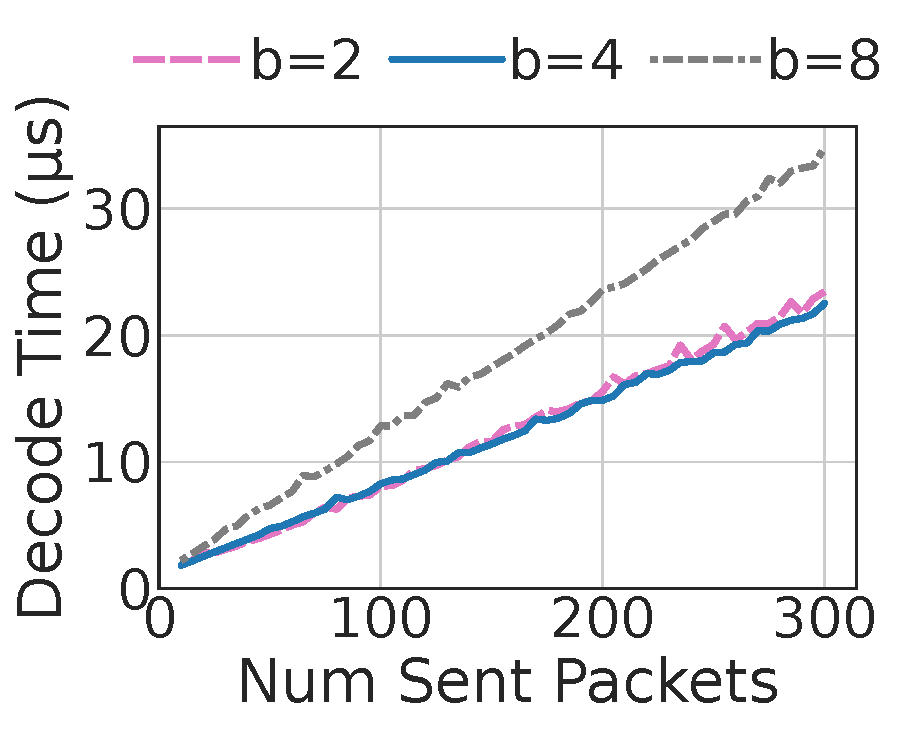
\includegraphics[width=\linewidth,trim={3mm 0 7mm 0},clip]{sidekick-paper/figures/fig2a_quack_num_candidates_vs_decode_time.pdf}
	\caption{\footnotesize Evaluate a degree-$m=t=10$ polynomial at $n$ candidate roots.}
	\label{fig:n-vs-decoding}
\end{subfigure}
\hspace{-0.1em}
\begin{subfigure}{0.32\columnwidth}
	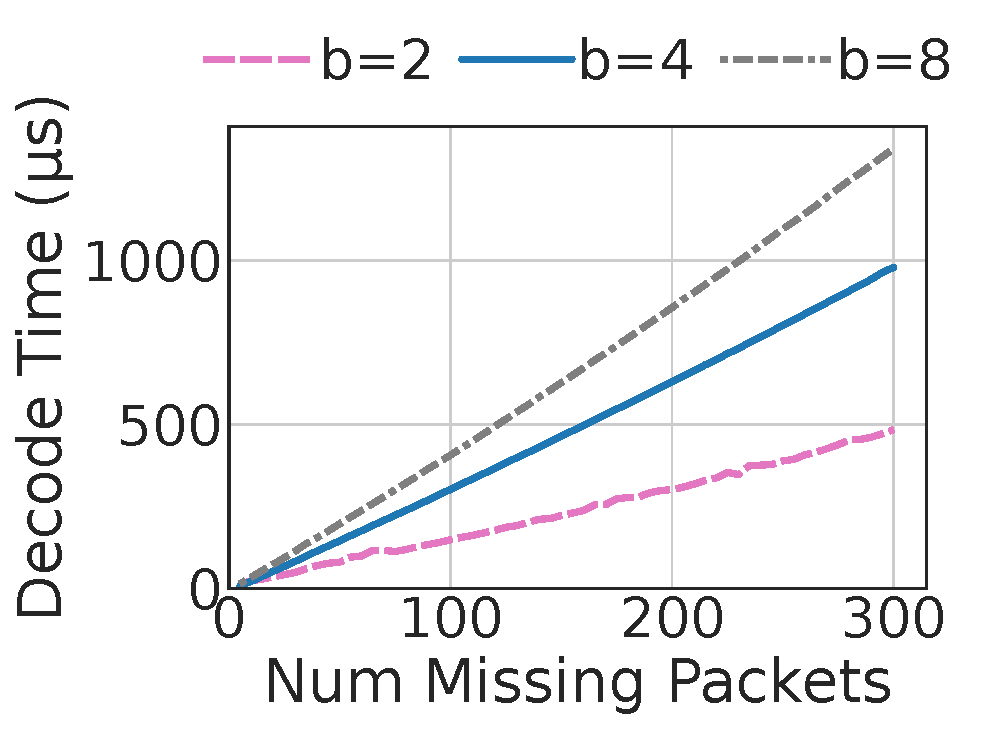
\includegraphics[width=\linewidth,trim={3mm 0 7mm 0},clip]{sidekick-paper/figures/fig2b_quack_num_missing_vs_decode_time.pdf}
	\caption{\footnotesize Plug $n=300$ candidate roots into a degree-$m$ polynomial.}
	\label{fig:m-vs-decoding}
\end{subfigure}
\hspace{-0.1em}
\begin{subfigure}{0.32\columnwidth}
	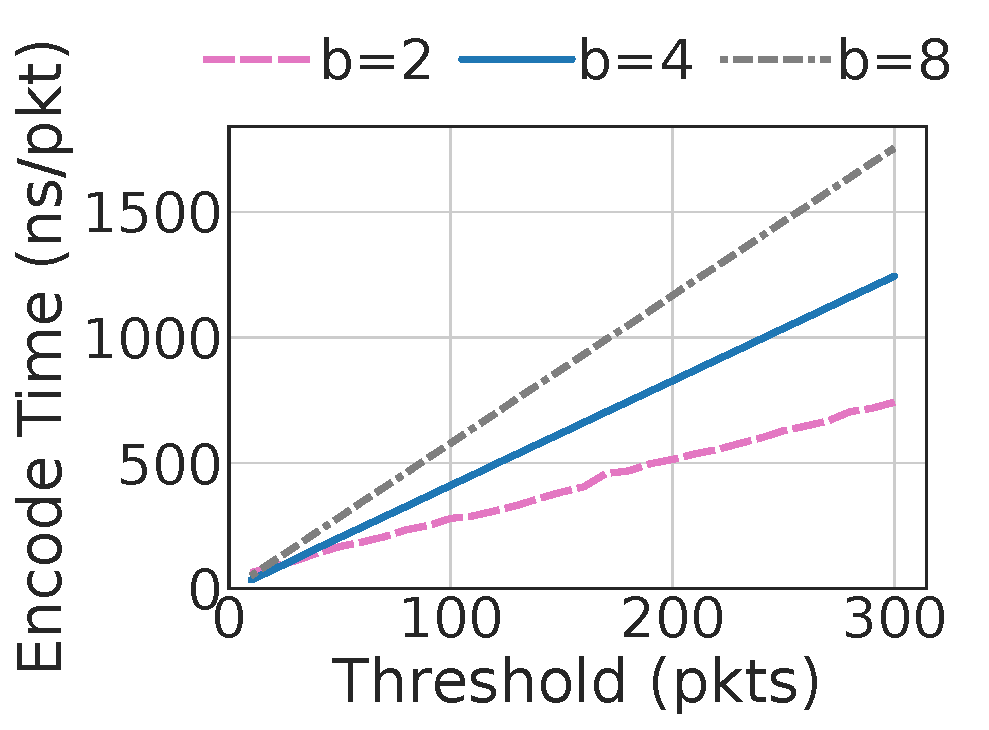
\includegraphics[width=\linewidth,trim={3mm 0 7mm 0},clip]{sidekick-paper/figures/fig2c_quack_threshold_vs_encode_time.pdf}
	\caption{\footnotesize Update $t$ power sum equations.
	Average of $1000$ packets.}
	\label{fig:construction-time}
\end{subfigure}
\vspace{-0.2cm}
\caption{How power sum quACK performance depends on various parameters:
bit width, threshold, number of sent and missing packets.
Average of 100 trials.
\vspace{-0.5cm}
}
\label{fig:quack-plots}
\end{figure}


\subsection{Identifier bit widths}
\label{sec:quack:microbenchmarks:bit-widths}

Different bit widths have different implications for
which instructions the CPU can use. Modular operations are efficient
for 16- and 32-bit integers, fitting within the 64-bit word size (the number of
bits that can be processed in one instruction) of most modern CPUs. For example,
to multiply two 32-bit integers, we cast them to 64-bit integers, multiply,
then take the modulus.

\Cref{fig:quack-plots} shows the best performance we achieved at different bit
widths. For 16-bit identifiers only, we precomputed power tables that fit in
the L3 cache. For 64-bit identifiers, we implemented Montgomery modular
multiplication~\cite{montgomery1985modular} to avoid an expensive hardware
division for 128-bit integers. In the remainder of the paper, we use $b=4$ as
the preferred tradeoff between space and collision probability.

\subsection{Encoding time}
\label{sec:quack:microbenchmarks:encoding}

The encode time per-packet is directly proportional to
the threshold number of missing packets $t$ (\Cref{fig:construction-time}) at
$33/10 \approx 3$ ns/power sum.
Each power sum can be updated in a constant number of operations based on the
previous power sum, so encoding an identifier requires $t$ modular additions
and multiplications for the $t$ power sums.

Encoding in the IBLT is faster in practice when there are at least
$\approx\!30$ symbols (\Cref{fig:quack:encode}).
Each update in the IBLT uses an expensive square root instruction in the
pseudorandom mapping algorithm, adding constant factor overheads that impact
smaller numbers of symbols.

\subsection{Decoding time}
\label{sec:quack:microbenchmarks:decoding}

The decode time must be comparable to the time it takes to process a typical
ACK and modify the logic in the transport protocol. Decoding typically
occurs on end hosts, compared to encoding which occurs in the middle of the path.

Finding the solution to the system of power sum polynomial equations boils down
to applying Newton's identities (a linear algorithm) and finding the roots of a
polynomial equation
in a modular field~\cite{eppstein2011straggler}.
Factoring a polynomial is asymptotically fast in theory, but the implementation
is branch-heavy and complicated~\cite{batut2000user}.
We found that plugging in and evaluating which of $n$ candidate roots
evaluated to zero was faster in practice for $n < 40,000$ roots.
This is the method we use to decode the power sum quACK.

The decode time of this method is directly proportional to $n$ (\Cref{fig:n-vs-decoding})
and the number of missing packets $m$ (\Cref{fig:m-vs-decoding}).
Decoding takes $2820/10/25 \approx 11$ ns/candidate/missing.
Both $n$ and $m$ are typically a few hundred at most.

Decoding in the IBLT is much faster in practice for any number of symbols
(\Cref{fig:quack:decode}). Note that the power sum quACK actually uses a decoding
method that is linear in \textit{all} packets received, not just the \textit
{missing} packets, due to the complexity of symmetric polynomial
factorization.

\subsection{IBLT non-determinism}
\label{sec:quack:microbenchmarks:non-determinism}

\begin{figure}[t]
    \centering
    \begin{subfigure}[b]{0.49\linewidth}
        \centering
        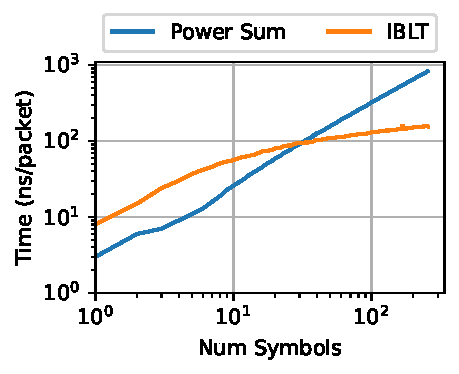
\includegraphics[width=\linewidth]{figures/quack_encode.pdf}
        \caption{Encode time.}
        \label{fig:quack:encode}
    \end{subfigure}
    \begin{subfigure}[b]{0.49\linewidth}
        \centering
        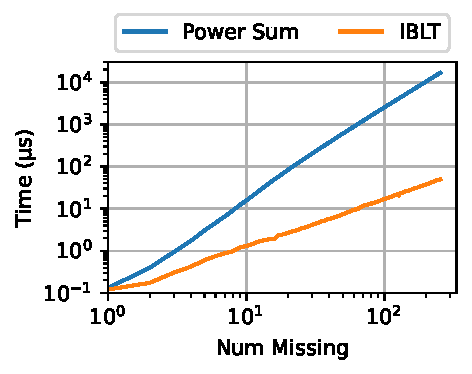
\includegraphics[width=\linewidth]{figures/quack_decode.pdf}
        \caption{Decode time.}
        \label{fig:quack:decode}
    \end{subfigure}
    \caption{IBLT vs. power sum eACK microbenchmarks. The number of trials is
     such that the cumulative time is at least $100$ ms. With rateless eACKs,
     the client can encode much larger numbers of symbols $t$ while the proxy
     decodes fewer symbols in the common case.
     % The logscale axes emphasize the overheads at smaller numbers.
     }
    \label{fig:quack}
\end{figure}
\begin{figure}[t]
    \centering
    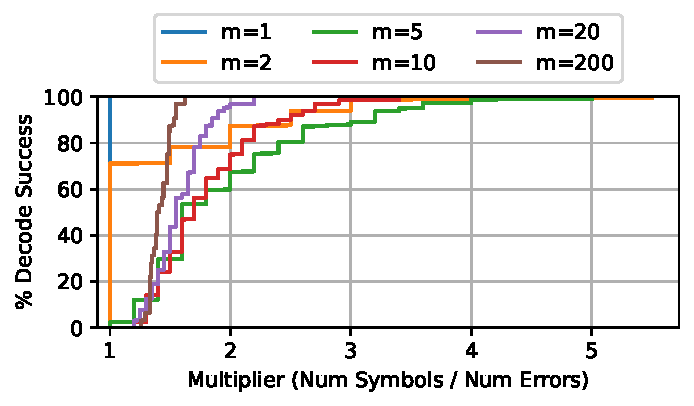
\includegraphics[width=0.9\linewidth]{packrat-paper/figures/quack_multiplier.pdf}
    \caption{The CDF of the minimum number of symbols $t$ needed to successfully
    decode an quACK for various numbers of missing packets $m$, 100000 trials.}
    \label{fig:iblt-quack}
\end{figure}

It is unknown how many symbols are required in the IBLT to decode the same
number of $m$ missing packets using power sums in the previous benchmarks.
There is a constant factor overhead ($1.35\times$ on average~\cite
{yang2024practical}).
\Cref{fig:iblt-quack} shows the CDF of the minimum number of symbols to decode
various $m$ as this constant multiplier increases. $m=1$ trivially requires
one symbol, while the multiplier decreases for higher $m$ to achieve the same
success rates.

The quACK sender does not know how many symbols it needs to encode to later
decode a certain $m$. Using power sums, this is exactly $m$ symbols. In
the quACK, $4 \cdot m$ symbols have at least a $\!98.8\%$ success rate for
all $m$ evaluated in \Cref{fig:iblt-quack}. When $m$ is large, the quACK utilizes more
of the link, but maintaining more symbols at the proxy and client means
the Packrat has a greater worst-case tolerance for errors with the same encoding
overheads. The Packrat proxy can reset the connection if it cannot decode a quACK.

\section{Summary}
\label{sec:quack:summary}

\section{Implementation}
\label{sec:implementation}

\begin{table}[ht]
  \centering
  \begin{tabular}{l r r}
    \hline
    \textbf{Module} & \textbf{Language} & \textbf{LOC} \\
    \hline
    QuACK library (\Cref{sec:quack:microbenchmarks}) & Rust & 1772 \\
    Media server/client + integration & Rust & 478 \\
    \texttt{quiche} client integration & Rust & 1821 \\
    \texttt{libcurl} client integration & C & 1459 \\
    Proxy Sidekick binary & Rust & 833 \\
    \hline
  \end{tabular}
  \caption{Lines of code.
  }
  \label{tab:lines-of-code}
\end{table}


We now describe our implementation of Robin~\cite{sidekick-github} for several applications.
We integrated \sys functionality with a simple media client for low-latency streaming
and an HTTP/3 (QUIC) client.
The total implementation of the quACK library, and proxy and client
integrations used 6363 LOC (\Cref{tab:lines-of-code}).

% \paragraph{QuACK library.}
% Quack library.

\subsection{Baselines and Applications}

The baselines we evaluated against were the performance of two opaque transport
protocols without proxy assistance, and the fairness of a split CUBIC connection.

\paragraph{Low-latency media application.}
We implemented a simple server and client in Rust for streaming low-latency
media. The client sends a numbered packet containing 240 bytes of data every
20 milliseconds, representing an audio stream at 96 kbit/s.
The sequence number is encrypted on the wire.

The server receives packets. If it receives a nonconsecutive sequence number,
it sends a NACK back to the client that contains the sequence number of each
missing packet. The client's behavior on NACK is to retransmit the packet. The
server retransmits NACKs, up to one per RTT, until it has received the packet.

The server's application behavior is to store incoming packets in a buffer
and play them as soon as the next packet in the sequence is available. The
de-jitter buffer delay is the length of time between when the packet is stored
to when it can be played in-order. Some packets can be played immediately.

\paragraph{HTTP/3 file upload application.}
We used the popular \texttt{libcurl}~\cite{libcurl} file transfer library as the basis for
our HTTP client, and an \texttt{nginx} webserver. The client makes an HTTP
POST request to the server. Both are patched with \texttt{quiche}~\cite{quiche}, a production
implementation of the QUIC protocol from Cloudflare, to provide support for
HTTP/3.

For our TCP baselines, we used the same file upload application with the
default HTTP/1.1 server and client. We used a split-connection
TCP PEP~\cite{caini2006pepsal} that intercepts the TCP
SYN packet in the three-way handshake, pretends to be the other side of that
connection, and initiates a new connection to the real endpoint.
Both clients use CUBIC congestion control.

\subsection{Client Integration}

In each application, we modified only the \emph{client} to speak Robin
and respond to in-network feedback. The server remained unchanged.
The modifications were in two parts: following the discovery mechanism to
establish bi-directional communication with the proxy, and using the information
in the quACK to modify transport layer behavior.

\begin{table*}[t]
  \centering
  % \renewcommand{\arraystretch}{0.000023}
  \begin{tabular}{lllll}
    \toprule
    & \bf Data Sender  & \bf Proxy $\leftrightarrow$ Data & \bf QuACK     & \bf Num \\
    & \bf (Client) $\leftrightarrow$ Proxy & \bf Receiver (Server) & \bf Interval & \bf Symbols \\
    \midrule
    \#1 Low-latency media & $1$ms, $100$ Mbit/s, & $25$ms, $10$ Mbit/s, & $2$ pkts & $8$ \\
                          & $3.6\%$ loss         & $0\%$ loss           &          &     \\

    \#2 Connection-splitting & $1$ms, $100$ Mbit/s, & $25$ms, $10$ Mbit/s, & $30$ ms & $10$ \\
    PEP emulation            & $1.0\%$ loss         & $0\%$ loss           &         & \\

    \#3 ACK reduction & $25$ms, $10$ Mbit/s, & $1$ms, $100$ Mbit/s & $15$ ms & $50$ \\
                      & $0\%$ loss,          & $0\%$ loss          &         & \\
    \bottomrule
  \end{tabular}
  \caption{Experimental scenarios. Link 1 connects the data sender (client) to
  the proxy, while Link 2 connects the proxy to the data receiver (server).
  The quACK interval and number of symbols represent our Sidekick configuration
  in the \texttt{Init} message.
  }
  \label{tab:sidekick:experimental-scenarios}
\end{table*}


% Recall that clients may respond to end-to-end ACKs in the following ways:
% \begin{enumerate}[noitemsep]
% 	\item Retransmit lost packets.
% 	\item Update the congestion window.
% 	\item Move the sending window.
% 	\item Forget packets in the retransmission buffer.
% \end{enumerate}
% \noindent They can similarly use quACKs to modify the base protocol, with the
% additional knowledge of \emph{where} loss occured.

\paragraph{Low-latency media client.} The media client has two open UDP sockets:
one for the base connection and one for the \sys connection. When it receives a
quACK, it detects lost packets without reordering and immediately retransmits
them. The protocol does not have a congestion window nor a flow-control window.
The client also sends reset and configuration messages over the \sys connection.

\paragraph{HTTP/3 file upload client.}
The HTTP/3 client similarly has an adjacent UDP socket for the \sys connection on
which it receives quACKs and sends reset and configuration messages. The client
passes the quACK to our modified \texttt{quiche} library, which interprets the
quACK and makes transport layer decisions. From the client's perspective,
\texttt{quiche} tells \texttt{libcurl} exactly what bytes to send over the wire.

Our modified \texttt{quiche} library uses the quACK to inform the
retransmission behavior, congestion window, and flow-control window. The library
immediately retransmits lost \emph{frames} in a newly-numbered
packet, as opposed to the lost \emph{packet}, similar to QUIC's original
retransmission mechanism. We implement PACUBIC,
described in \Cref{sec:design:cubic}.
We also move the flow-control window (without forgetting packets in the
retransmission buffer), but only in the ACK reduction scenario, when the
congestion window is nearly representative of that of the \sys connection's
path segment.

% For the \sys receiver, we augmented \texttt{quiche}~\cite{quiche}, a production
% implementation of the QUIC protocol from Cloudflare, and the popular
% \texttt{curl} HTTP/3 client patched with \texttt{quiche}.
% We modified 967 LOC in the \texttt{curl} C integration and
% 557 LOC in the \texttt{quiche} Rust integration.

% Over the course of working with quiche, we discovered and raised several bugs
% in the quiche implementation with its maintainers, including flow control
% limit negotiation, congestion window size calculation, and interpretations of
% the spec for detecting spurious loss congestion events [citations omitted].
% % \michael{should this be replaced with: ``removed for anonymity''?
% % Note, in this case, we should also remove the later text where you describe the spurious case in greater detail and again say that we pointed it out to the devs.}
% We are still able to show that quiche (and its CUBIC implementation) generally
% matches the behavior and performance of TCP end-to-end, but inevitably there
% will be differences due to the experimental nature of QUIC.

\subsection{Proxy Integration}
\label{sec:implementation:proxy}

Our proxy sniffs incoming packets of a network interface using the
\texttt{recvfrom} system call on a raw socket.
It stores a hash table using Rust's standard library \texttt{HashMap} that maps
socket pairs to their respective quACKs, and
incrementally updates the quACKs for flows that have requested \sys assistance.
It also sends quACKs at their configured frequencies and listens for
configuration messages.

% There are several alternative designs. The proxy could also parse packets
% directly from the kernel using, e.g., eBPF, or process packets directly in the
% data plane. These designs could be faster, but more difficult to implement.
% Instead of quACKing in a separate UDP stream, the proxy could piggyback quACKs
% onto the existing stream. However, this would depend on the message frequency
% in the base connection, and could also cause the packet size to exceed the MTU.

\section{Implementation}
\label{sec:sidekick:implementation}

\begin{table}[ht]
  \centering
  \begin{tabular}{l r r}
    \hline
    \textbf{Module} & \textbf{Language} & \textbf{LOC} \\
    \hline
    Media server/client + integration & Rust & 478 \\
    \texttt{quiche} client integration & Rust & 1821 \\
    \texttt{libcurl} client integration & C & 1459 \\
    Sidekick proxy binary & Rust & 833 \\
    \hline
  \end{tabular}
  \caption{Lines of code in the Sidekick protocol implementation.
  }
  \label{tab:sidekick:lines-of-code}
\end{table}


We now describe our implementation of the Sidekick protocol for several
applications. We integrated Sidekick functionality with a simple media client
for low-latency streaming and an HTTP/3 (QUIC) client. We used the power sum
construction of the quACK from our quACK library in \Cref
{sec:quack:implementation}. The total implementation of the proxy and client
integrations used 4591 LOC (\Cref{tab:sidekick:lines-of-code}).

\subsection{End-to-end applications}
\label{sec:sidekick:implementation:applications}

The baselines we evaluated against were the performance of two secure transport
protocols without proxy assistance, and the fairness of a split CUBIC connection.

\subsubsection{Low-latency media application.}
We implemented a simple server and client in Rust for streaming low-latency
media. The client sends a numbered packet containing 240 bytes of data every
20 milliseconds, representing an audio stream at 96 kbit/s.
The sequence number is encrypted on the wire.

The server receives packets. If it receives a nonconsecutive sequence number,
it sends a NACK back to the client that contains the sequence number of each
missing packet. The client's behavior on NACK is to retransmit the packet. The
server retransmits NACKs, up to one per RTT, until it has received the packet.

The server's application behavior is to store incoming packets in a buffer
and play them as soon as the next packet in the sequence is available. The
de-jitter buffer delay is the length of time between when the packet is stored
to when it can be played in-order. Some packets can be played immediately.

\subsubsection{HTTP/3 file upload application.}
We used the popular \texttt{libcurl}~\cite{libcurl} file transfer library as the basis for
our HTTP client, and an \texttt{nginx} webserver. The client makes an HTTP
POST request to the server. Both are patched with \texttt{quiche}~\cite{quiche}, a production
implementation of the QUIC protocol from Cloudflare, to provide support for
HTTP/3.

For our TCP baselines, we used the same file upload application with the
default HTTP/1.1 server and client. We used a split-connection
TCP PEP~\cite{caini2006pepsal} that intercepts the TCP
SYN packet in the three-way handshake, pretends to be the other side of that
connection, and initiates a new connection to the real endpoint.
Both clients use CUBIC congestion control.

\subsection{Client integrations with Sidekick}
\label{sec:sidekick:implementation:client-integrations}

In each application, we modified only the \emph{client} to speak the Sidekick
protocol and respond to in-network feedback. The server remained unchanged.
The modifications were in two parts: following the discovery mechanism to
establish bi-directional communication with the proxy, and using the information
in the quACK to modify transport layer behavior.

\begin{table*}[t]
  \centering
  % \renewcommand{\arraystretch}{0.000023}
  \begin{tabular}{lllll}
    \toprule
    & \bf Data Sender  & \bf Proxy $\leftrightarrow$ Data & \bf QuACK     & \bf Num \\
    & \bf (Client) $\leftrightarrow$ Proxy & \bf Receiver (Server) & \bf Interval & \bf Symbols \\
    \midrule
    \#1 Low-latency media & $1$ms, $100$ Mbit/s, & $25$ms, $10$ Mbit/s, & $2$ pkts & $8$ \\
                          & $3.6\%$ loss         & $0\%$ loss           &          &     \\

    \#2 Connection-splitting & $1$ms, $100$ Mbit/s, & $25$ms, $10$ Mbit/s, & $30$ ms & $10$ \\
    PEP emulation            & $1.0\%$ loss         & $0\%$ loss           &         & \\

    \#3 ACK reduction & $25$ms, $10$ Mbit/s, & $1$ms, $100$ Mbit/s & $15$ ms & $50$ \\
                      & $0\%$ loss,          & $0\%$ loss          &         & \\
    \bottomrule
  \end{tabular}
  \caption{Experimental scenarios. Link 1 connects the data sender (client) to
  the proxy, while Link 2 connects the proxy to the data receiver (server).
  The quACK interval and number of symbols represent our Sidekick configuration
  in the \texttt{Init} message.
  }
  \label{tab:sidekick:experimental-scenarios}
\end{table*}


\paragraph{Low-latency media client.} The media client has two open UDP sockets:
one for the base connection and one for the Sidekick connection. When it receives a
quACK, it detects lost packets without reordering and immediately retransmits
them. The protocol does not have a congestion window nor a flow-control window.
The client also sends reset and configuration messages over the Sidekick connection.

\paragraph{HTTP/3 file upload client.}
The HTTP/3 client similarly has an adjacent UDP socket for the Sidekick connection on
which it receives quACKs and sends reset and configuration messages. The client
passes the quACK to our modified \texttt{quiche} library, which interprets the
quACK and makes transport layer decisions. From the client's perspective,
\texttt{quiche} tells \texttt{libcurl} exactly what bytes to send over the wire.

Our modified \texttt{quiche} library uses the quACK to inform the
retransmission behavior, congestion window, and flow-control window. The library
immediately retransmits lost \emph{frames} in a newly-numbered
packet, as opposed to the lost \emph{packet}, similar to QUIC's original
retransmission mechanism. We implement PACUBIC,
described in \Cref{sec:sidekick:sender}.
We also move the flow-control window (without forgetting packets in the
retransmission buffer), but only in the ACK reduction scenario, when the
congestion window is nearly representative of that of the Sidekick connection's
path segment.

\subsection{Sidekick proxy}
\label{sec:sidekick:implementation:proxy}

Our proxy sniffs incoming packets of a network interface using the
\texttt{recvfrom} system call on a raw socket.
It stores a hash table using Rust's standard library \texttt{HashMap} that maps
socket pairs to their respective quACKs, and
incrementally updates the quACKs for flows that have requested Sidekick assistance.
It also sends quACKs at their configured frequencies and listens for
configuration messages.

\section{Evaluation methodology}
\label{sec:sidekick:methodology}

\begin{figure}[t]
\centering
\includegraphics[width=0.7\linewidth]{sidekick/figures/setup_real.pdf}
\caption{Real-world experimental setup.
}
\label{fig:sidekick:real-setup}
\end{figure}


We modeled the scenarios from \Cref{sec:sidekick:motivating}. We use the same
m4.xlarge AWS instance as before for the emulated experiments.

\subsubsection{Emulation experiments.}

We emulated a two-hop network topology (\Cref{fig:sidekick:overview}) in mininet,
configuring the link properties using \texttt{tc}.
In emulation, we represented
each link by a constant delay (with variability induced by the queue), a random
loss percentage, and a maximum bandwidth.
\Cref{tab:sidekick:experimental-scenarios} describes the parameters
for each link to model---e.g., lossy Wi-Fi or a high-latency cellular
path---as well as the metrics for success in that scenario.
Link 1 connects the data sender (client) to the proxy,
while Link 2 connects the proxy to the data receiver (server).
On the proxy, we either run a Sidekick,
a connection-splitting TCP PEP~\cite{caini2006pepsal}, or nothing at all.

\subsubsection{Real-world experiments.}

To test its robustness, we also evaluated the Sidekick protocol over a real-world
environment that resembled the scenario on the train (\Cref{fig:sidekick:real-setup}).
In this setup, a Lenovo ThinkPad laptop, running Ubuntu 22.04.3 with a 4-Core
Intel i7 CPU @ 2.60 GHz and 16 GB memory, acted as a client to an AWS instance in
the nearest geographical region. The ThinkPad used as an access point (AP)
a Lenovo Yoga laptop, running Ubuntu 20.04.6 with a 4-Core Intel i5 CPU @
1.60 GHz and 4 GB memory, with a 2.4 GHz Wi-Fi hotspot.
The AP was connected to the Internet via a JEXtream cellular modem
with a 5G data plan. The AP ran Sidekick software.

We measured the link properties of each path segment to compare to
our emulation parameters. We measured delay and loss using 1000~\texttt{ping}s
over a 100 second period, and bandwidth using an \texttt{iperf3} test.
On the near segment between the ThinkPad client and the AP,
the min/avg/max/stdev RTT was 1.249/37.194/272.168/54.660 ms
at 49.8 Mbit/s bandwidth. We observed that loss increased
the further away the AP. In our experiments, the client was located roughly
200 feet away in a different room, with 3.6\% loss.
The far segment between the AP and the AWS server was
48.546/64.381/92.374/6.806 ms with 0.0\% loss at 30.9 Mbit/s.
In both environments, the cellular link was the bottleneck link in terms of
bandwidth, and the corresponding path segments in emulation had similar
minimum RTTs and average loss percentages.

\section{Real-world results}
\label{sec:sidekick:real-world}

\begin{figure}[t]
\centering
\begin{subfigure}{0.48\linewidth}
	\includegraphics[width=\linewidth]{sidekick/figures/fig8_real_world_webrtc.pdf}
	\caption{Low-latency media. CDF of per-packet de-jitter
	latencies over 10 one-minute trials per protocol.}
	\label{fig:sidekick:real-world:media}
\end{subfigure}
\begin{subfigure}{0.48\linewidth}
	\includegraphics[width=\linewidth]{sidekick/figures/fig8_real_world_retx.pdf}
	\caption{Path-aware congestion control.
	Median of 20 trials. Error bars are 1st and 3rd quartiles.}
	\label{fig:sidekick:real-world:pep-emulation}
\end{subfigure}
\caption{Real-world results. Experiments were run in a moderately well-attended
office environment over a Friday afternoon. Trials alternate between the
baseline and the Sidekick to account for variability in time of day.
}
\label{fig:sidekick:real-world}
\end{figure}


We discuss the results of our experiments replicating two of our scenarios in
the real world, using as context
these main differences between emulation and the real-world:

\begin{itemize}[noitemsep,topsep=0pt]
  \item The RTT is more variable as it depends on interactions in the
  wireless medium and the shared cellular path.
  \item Wireless loss can be more variable as nearby 2.4 GHz devices and
  physical barriers may interfere with the link. Wireless loss also tends
  to be more clustered in practice.
  \item The available bandwidth on the shared cellular path is more variable,
  and depends on the time of day.
\end{itemize}

\Cref{fig:sidekick:real-world} shows the results of running the low-latency media and
connection-splitting PEP emulation experiments in the real-world. The baseline
protocol with a Sidekick is able to
reduce the 99th percentile de-jitter latency of an audio stream
from 2.3~seconds to 204~ms---about a 91\% reduction---and
improve the goodput of a 50 MB HTTP/3 upload by about 50\%.
Although the improvements are more conservative compared to emulation in
\Cref{fig:sidekick:main-results:media} and
\Cref{fig:sidekick:main-results:pep-emulation}, each case still benefits the
base protocol under all circumstances, compared to end-to-end mechanisms alone.

Part of the difference can be attributed to the network setting. When there is
no loss on the near path segment, as can occasionally happen in a real Wi-Fi link,
we do not expect to
see a difference with a Sidekick. When there is more loss on the far path segment, which
is variable and depends on the time, we
expect the benefit of the Sidekick to be less since this equally affects the
performance of the base protocol.

The other part of the difference could be made up by future work that better
adapts a Sidekick connection to real-world variability: The client could improve
path segment RTT estimation based on when the proxy receives packets, and use this
dynamic estimate in the calculation of $r$ used in $\beta$ and $C$.
The client could also use
this estimate to dynamically adjust the quACK interval.
Finally, we could analyze theoretically how PACUBIC responds
to traffic patterns in the real world.

\section{Emulation results}
\label{sec:sidekick:emulation}

\begin{figure*}
\begin{subfigure}{0.34\textwidth}
\includegraphics[width=\linewidth]{sidekick/figures/fig4a_low_latency_media.pdf}
\caption{Scenario \#1: Low-latency media.
 Reduced tail latency of de-jitter delay
with earlier retransmission. 5 minute trials.}
\label{fig:sidekick:main-results:media}
\end{subfigure}
\hfill
\begin{subfigure}{0.31\textwidth}
\includegraphics[width=0.97\linewidth]{sidekick/figures/fig4b_pep_emulation.pdf}
\caption{Scenario \#2: Connection-splitting PEP emulation. Improved goodput.
20 trials median. Error bars are 1st and 3rd quartiles.
}
\label{fig:sidekick:main-results:pep-emulation}
\end{subfigure}
\hfill
\begin{subfigure}{0.32\textwidth}
\includegraphics[width=0.99\linewidth]{sidekick/figures/fig4c_ack_reduction.pdf}
\caption{Scenario \#3: ACK reduction.
High goodput independent of end-to-end ACK frequency.
10 MB upload.}
\label{fig:sidekick:main-results:ack-reduction}
\end{subfigure}
\caption{
Comparing the end-to-end baseline protocol to the same protocol with a Sidekick
connection, using the success metrics for the three scenarios described in
\Cref{tab:sidekick:experimental-scenarios}. The \textsf{Sidekick($N$x)} data points show
the performance at $N$x the quACK interval (sent less frequently) and
threshold of the default configurations specified in
\Cref{tab:sidekick:experimental-scenarios}.
}
% \dm{Maybe a notation like $x/4$ would be more suggestive than $4x$?}
\label{fig:sidekick:main-results}
\end{figure*}


We evaluated our implementation of the Sidekick protocol in a more controlled
emulation environment to answer the following questions:
\begin{enumerate}[noitemsep,topsep=0pt]
	\item Can Sidekicks improve the performance of secure transport protocols
	in a variety of scenarios while preserving the end-to-end behavior of the
	base protocols?
	\item Can a path-aware congestion control algorithm match the fairness of
	split TCP PEPs using CUBIC?
	\item How do the CPU overheads of encoding quACKs impact the maximum
	capacity of a proxy with a Sidekick?
	\item What link overheads does the power sum quACK add and how does it
	compare to the strawmen?
\end{enumerate}

\subsection{Performance of secure transport protocols with Sidekick}
\label{sec:sidekick:emulation:performance}

We first evaluate Sidekick's main performance goal: In each of the motivating
scenarios, we show that the Sidekick protocol can improve performance compared
to the base protocol alone, which would not be able to benefit from existing
PEPs. Each scenario has a different metric for success---tail latency,
throughput, or number of packets sent by the data receiver (corresponding to
energy usage or chance of Wi-Fi collisions)---demonstrating the versatility of
the Sidekick protocol.

\subsubsection{Low-latency media application.}
The Sidekick can reduce tail latencies in a low-latency media stream, representing
fewer drops and better quality of experience.
The early retransmissions induced by the Sidekick reduced the 99th percentile
latency of the de-jitter buffer delay from 48.6 ms to 2.2 ms---a 95\%
reduction (\Cref{fig:sidekick:main-results:media}).
As long as the quACK interval is less than the end-to-end RTT, the connection
benefits from the Sidekick.

The Sidekick is beneficial in this scenario because it enables the client to sooner
detect and retransmit lost packets, and the server to sooner play packets from
its de-jitter buffer.
The end-to-end mechanism takes one additional received packet to notify of the
loss and
one end-to-end RTT to retransmit and play the packet (20+52=72ms), resulting in
three delayed packets (the three ``steps" in \Cref{fig:sidekick:main-results:media}) in most cases.
The Sidekick takes up to two additional packets and one near path segment RTT
(20+2=22ms or 20$\times$2+2=42ms), delaying either one or two packets in comparison.
Dropped ACKs and quACKs account for the $<2\%$ of packets with even greater
de-jitter latencies.

\subsubsection{Connection-splitting PEP emulation.}
The Sidekick improves upload speeds when there is a lossy, low-latency link
by using quACKs to inform the sender's congestion control.
In a scenario with $1\%$ random loss on the link between the proxy and the
data sender, the HTTP/3 (QUIC) client achieves $3.6\times$ the goodput for a 10 MB
upload with a Sidekick compared to end-to-end QUIC (\Cref{fig:sidekick:main-results:pep-emulation}).

When there is no random loss, the Sidekick does not impact the performance
of QUIC\@.
There are no logical changes to the base protocol in this case because all loss
is on the
bottleneck link on the far path segment, and the CPU overheads of processing quACKs
are negligible.

Knowing \emph{where} congestion occurs is an opportunity for creating smarter
congestion control. In PACUBIC, identifying where the loss occured let the data
sender reduce the congestion window proportionally to how many packets were
in-flight on each path segment. In \Cref{sec:sidekick:emulation:pacubic}, we
will show that our path-aware congestion control algorithm still matches the
fairness of connection-splitting TCP PEPs.

\subsubsection{ACK reduction scenario.}

Using quACKs in lieu of end-to-end ACKs allows the data receiver to
significantly reduce its ACK frequency while maintaining high goodput.
In our experiment, QUIC with a Sidekick sent $96\%$ fewer packets (mainly ACKs)
than end-to-end QUIC before the goodput dropped below 8.5 Mbit/s
(\Cref{fig:sidekick:main-results:ack-reduction}).
The quACK enables the data sender to promptly move the flow-control window forward,
as long as the last hop is reliable.

The goodput significantly degrades when reducing the end-to-end ACK frequency
without a Sidekick. When end-to-end QUIC reduces the ACK frequency to every
80 ms, the data receiver sends $247 / 138 = 1.8\times$ the packets at
$4.5 / 8.4 = 0.5\times$ the goodput, worse than QUIC with the Sidekick
in both dimensions (\Cref{fig:sidekick:main-results:ack-reduction}). With a Sidekick,
the data sender also does not need to change packet pacing to avoid bursts in
response to infrequent ACKs, which is why end-to-end QUIC cannot send fewer
than $\approx 240$ packets.

\subsubsection{Discussion: Configuring the Sidekick connection.}
\Cref{tab:sidekick:experimental-scenarios} shows the quACK interval and threshold we
elected for each scenario based on the considerations in
\Cref{sec:sidekick:init}. In each experiment in \Cref{fig:sidekick:main-results},
we also show how with less frequent quACKs ($2\times$ and $4\times$ the
interval) and proportionally-adjusted thresholds, the protocol performs worse,
or more variably. Less frequent quACKs means the client reacts later to
feedback about the near path segment, and more often has to rely on the
end-to-end mechanism. The performance particularly degrades when the quACK
interval exceeds the end-to-end RTT. However, even in this case, the base
protocol with any Sidekick at all performs better than the base protocol alone\@.

\subsection{Link overheads from sending quACKs}
\label{sec:sidekick:emulation:link-overheads}

\begin{table}[ht]
\begin{subtable}{\columnwidth}
  \setlength{\tabcolsep}{2pt}
  \centering
  \begin{tabular}{lccccccc}
    \toprule
    & \multicolumn{2}{c}{Data Sender$\rightarrow$} & \multicolumn{2}{c}{$\leftarrow$Proxy} & \multicolumn{2}{c}{$\leftarrow$Data Receiver} & \\
    & \bf Pkts & \bf Bytes & \bf Pkts & \bf Bytes & \bf Pkts & \bf Bytes & \bf Goodput \\
    \midrule
    QUIC E2E & $1.00\times$ & $1.00\times$ & $1.00\times$ & $1.00\times$ & $1.00\times$ & $1.00\times$ & $1.00\times$ \\
    Strawman 1a & $0.96\times$ & $1.01\times$ & \cellcolor{LighterRed}{$2.02\times$} & \cellcolor{LightestRed}{$1.56\times$} & $1.01\times$ & $1.03\times$ & \cellcolor{LighterGreen}{$3.33\times$} \\
    Strawman 1b & $0.94\times$ & $1.00\times$ & \cellcolor{LighterRed}{$2.00\times$} & \cellcolor{LightestRed}{$1.78\times$} & $1.00\times$ & $1.03\times$ & \cellcolor{LightGreen}{$3.53\times$} \\
    Strawman 1c & \cellcolor{LightestRed}{$1.83\times$} & $1.06\times$ & \cellcolor{LighterRed}{$2.01\times$} & \cellcolor{LightestRed}{$1.83\times$} & $1.00\times$ & $1.03\times$ & \cellcolor{LightGreen}{$3.46\times$} \\
    \bf \textcolor{black!50!blue}{Power Sum}   & \textcolor{black!50!blue}{\bf 0.94$\times$} & \textcolor{black!50!blue}{\bf 1.00$\times$} & \textcolor{black!50!blue}{\bf 1.03$\times$} & \textcolor{black!50!blue}{\bf 1.07$\times$} & \textcolor{black!50!blue}{\bf 1.00$\times$} & \textcolor{black!50!blue}{\bf 1.03$\times$} & \cellcolor{LightGreen}{\textcolor{black!50!blue}{\bf 3.55$\times$}} \\
    \bottomrule
  \end{tabular}
  \caption{Scenario \#2: Connection-splitting PEP emulation.\\}
  \label{tab:sidekick:packet-overheads:retx}
\end{subtable}
\begin{subtable}{\columnwidth}
  \setlength{\tabcolsep}{2pt}
  \centering
  \begin{tabular}{lccccccc}
    \toprule
    & \multicolumn{2}{c}{Data Sender$\rightarrow$} & \multicolumn{2}{c}{$\leftarrow$Proxy} & \multicolumn{2}{c}{$\leftarrow$Data Receiver} & \\
    & \bf Pkts & \bf Bytes & \bf Pkts & \bf Bytes & \bf Pkts & \bf Bytes & \bf Goodput \\
    \midrule
    QUIC E2E & $1.00\times$ & $1.00\times$ & $1.00\times$ & $1.00\times$ & $1.00\times$ & $1.00\times$ & $1.00\times$ \\
    Strawman 1a & $0.96\times$ & $1.00\times$ & \cellcolor{LightRed}{$9.94\times$} & \cellcolor{LighterRed}{$4.99\times$} & \cellcolor{LightGreen}{$0.04\times$} & \cellcolor{LightGreen}{$0.08\times$} & $1.02\times$ \\
    Strawman 1b & $0.96\times$ & $1.00\times$ & \cellcolor{LightRed}{$9.95\times$} & \cellcolor{LightRed}{$7.13\times$}      & \cellcolor{LightGreen}{$0.04\times$} & \cellcolor{LightGreen}{$0.08\times$} & $1.02\times$ \\
    Strawman 1c & \cellcolor{LightestRed}{$1.91\times$} & $1.05\times$ & \cellcolor{LightRed}{$9.73\times$} & \cellcolor{LightRed}{$7.41\times$}      & \cellcolor{LightGreen}{$0.04\times$} & \cellcolor{LightGreen}{$0.08\times$} & $0.97\times$ \\
    \bf \textcolor{black!50!blue}{Power Sum}    & \textcolor{black!50!blue}{\bf 0.96$\times$} & \textcolor{black!50!blue}{\bf 1.00$\times$} & \textcolor{black!50!blue}{\bf 1.09$\times$} & \cellcolor{LighterRed}{\textcolor{black!50!blue}{\bf 2.56$\times$}} & \cellcolor{LightGreen}{\textcolor{black!50!blue}{\bf 0.04$\times$}} & \cellcolor{LightGreen}{\textcolor{black!50!blue}{\bf 0.08$\times$}} & \textcolor{black!50!blue}{\bf 0.98$\times$} \\
    \bottomrule
  \end{tabular}
  \caption{Scenario \#3: ACK reduction.}
  \label{tab:sidekick:packet-overheads:ackr}
\end{subtable}
\caption{Link overheads for a 10 MB upload. The cells represent the multiplier
relative to the end-to-end QUIC baseline for each type of quACK\@.
Lower is better for number of packets and bytes sent on a link.
Higher goodput is better. The power sum quACK achieves the success metric
for each scenario without incurring the link overheads of the strawmen.
We did not evaluate the contrived protocol in Scenario \#1.
}
\label{tab:sidekick:packet-overheads}
\end{table}


The other cost in terms of using Sidekick protocols is the additional data
sent by the proxy to the data sender.
Too many additional bytes use up bandwidth, and additional packets use
up CPU\@.
\Cref{tab:sidekick:packet-overheads} shows the number of packets and bytes sent at each
node comparing the strawmen and power sum quACK to no Sidekick connection at all.

Using power sum quACKs increases the packets sent from the proxy to the data
sender
by 3-9\%. These packets either consist mostly
of end-to-end ACKs which are sent every packet in \texttt{quiche}, or end-to-end
ACKs that have been replaced by quACKs in the ACK reduction scenario.
We did not evaluate Scenario \#1 because it is based
on a contrived protocol that lacks many of these features, and the link
overheads would not really make sense.

This overhead is representative of the CPU overhead at the client, since
quACKs and ACKs take a similar number of cycles to process. In an experiment
with Scenario \#2 during a period of $\approx90$k incoming packets, ACKs took on
average 26065 cycles to process while the quACKs took 26369 cycles, 1\% more.
These cycles come from, i.e., the complex recovery and loss detection algorithms
implemented at the end host.

The strawmen have significantly higher link overheads compared to the power sum
quACK\@. The proxy sends up to 10$\times$ more packets using Strawman 1a, and
also slightly harms the goodput in the congestion control scenario.
The reduced goodput is due to the sender mis-identifying received packets as
dropped due to dropped quACKs.
The proxy achieves higher goodput with Strawman 1b but sends
more bytes. Strawman 1c increases the link overheads at both the proxy and the
data sender due to larger TCP headers and TCP ACKs.
We did not evaluate Strawman 2 due to its impractical decode time.

\subsection{CPU overheads of encoding at the proxy}
\label{sec:sidekick:emulation:cpu-overheads}

\begin{table}[ht]
  \centering
  \begin{tabular}{lrrrr}
    \toprule
    & \multicolumn{2}{r}{\bf 25-Byte Payload} & \multicolumn{2}{r}{\bf 1468-Byte Payload}\\
    & \bf Cycles & \bf $\%$ & \bf Cycles & \bf $\%$ \\
    \midrule
    Sniff Packet & 22417 & 97.6 & 22408 & 97.5 \\
    Table Lookup &   247 &  1.1 &   251 &  1.1 \\
    Parse ID     &    23 &  0.1 &    22 &  0.1 \\
    Encode ID    &    74 &  0.3 &    69 &  0.3 \\
    Other        &   213 &  0.9 &   225 &  1.0 \\
    \midrule
    \emph{Total} & \emph{22974} & \emph{100.0} & \emph{22975} & \emph{100.0} \\
    \bottomrule
  \end{tabular}
  \caption{Breakdown of the CPU cycles spent processing each packet at the
  proxy. Most cycles are spent on general per-packet overheads as opposed to
  quACK-specific processing.
  }
  \label{tab:sidekick:cpu-overheads}
\end{table}


The main bottleneck of Sidekick on a proxy is the CPU\@.
\Cref{tab:sidekick:cpu-overheads} shows a breakdown of the number of CPU cycles in each
step. The largest overhead was reading the packet contents from the network
interface ($97.5\%$ of the CPU cycles).

Encoding an identifier in a power sum quACK with $t=10$ used $74$ CPU
cycles ($0.9\%$). As a calculation of the theoretical maximum on a 2.30 GHz
% 2.30e9 / 74 = 31 million
CPU, the proxy would be able to process $31$ million packets/second on a single
core. The hash table lookup used $251$ cycles and parsing the pseudorandom
payload as an identifier used $22$ cycles.

In practice, we measured the maximum throughput of our Sidekick proxy to
be 464k packets/s with 25-byte payloads and 5.5 Gbit/s (458k packets/s) with
1468-byte packet payloads on a single core (assuming 1500-byte MTUs).
This experiment used multiple \texttt{iperf3} clients to simulate high
load until the proxy was unable to keep up with the load on a single core.
The packet payload size did not seem to affect results.

We find these achieved throughputs acceptable for edge routers such as Wi-Fi APs
and base stations. To deploy the Sidekick proxy on core routers, we would need
to reduce the overhead of reading packets from the NIC, such as by bypassing
the kernel/user-space protection boundary\footnote{ A kernel-bypass system like
Retina~\cite{wan2022retina} can achieve 25 Gbps on 2 cores while processing raw
packets with a 1000-cycle callback(Figure 5(a) in \cite{wan2022retina}). The
Sidekick equivalent would be a 500-cycle callback, and assuming all traffic has
requested Sidekick help. Throughput scales almost linearly with the number of
cores using symmetric RSS hashing. Thus we don't expect proxy overheads to be
an issue with modern 100 Gbps network speeds and an optimized implementation
even on commodity hardware. }~\cite{dpdk,mccanne1993bsd,wan2022retina} or using
native hardware~\cite{bosshart2014p4}. We could also scale on multiple cores
using symmetric RSS hashing~\cite{woo2012scalable}.

\subsection{TCP friendliness of path-aware CUBIC}
\label{sec:sidekick:emulation:pacubic}

\begin{figure}[t]
\centering

\includegraphics[width=\columnwidth]{sidekick/figures/fig5_baseline_bar_legend.pdf}
\begin{subfigure}{0.49\linewidth}
	\includegraphics[width=\linewidth]{sidekick/figures/fig5_baseline_loss0p.pdf}
	\caption{0\% loss.}
	\label{fig:sidekick:fairness-bar:loss0p}
\end{subfigure}
\begin{subfigure}{0.49\linewidth}
	\includegraphics[width=\linewidth]{sidekick/figures/fig5_baseline_loss1p.pdf}
	\caption{1\% loss.}
	\label{fig:sidekick:fairness-bar:loss1p}
\end{subfigure}
\caption{Median goodput for three upload data sizes with $0\%$ and $1\%$ loss on
Link 1. 20 trials. Error bars are 1st and 3rd quartiles.
With proxy assistance at $1\%$
loss, both QUIC and TCP match the performance of when there is no loss at all.
}
\label{fig:sidekick:fairness-bar}
\end{figure}

\begin{figure}[t]
\centering

\includegraphics[width=0.8\columnwidth]{sidekick/figures/fig6_legend.pdf}
\includegraphics[width=0.8\columnwidth]{sidekick/figures/fig6_loss_bw100_10M_delay_25ms_1ms.pdf}
\caption{Connection-splitting PEP emulation as a function of near-segment
	loss rate. In this emulation experiment, QUIC+Sidekick (running PACUBIC)
  performs similarly to TCP+PEP (each connection running CUBIC)
  and improves goodput compared with end-to-end protocols. The graph shows
  median goodput of a 10~MByte upload. QuACK interval is 30~ms, threshold
is 10. Error bars show IQR of 10 trials.
}
\label{fig:sidekick:fairness-line}
\end{figure}


It is easy to improve performance without regard to competing flows;
however, we demonstrate that PACUBIC can
match the fairness of split CUBIC in a TCP PEP connection\@.
We evaluate fairness using Scenario \#2 with varying amounts of loss on the
near path segment.

\subsubsection{QUIC vs.\ TCP\@.}
We first compare QUIC to TCP without either PEP\@.
As both connections use CUBIC, they exhibit similar
congestion control behavior and achieve nearly maximum throughput in the
emulated network with no random loss (\Cref{fig:sidekick:fairness-bar:loss0p}).
We attribute the differences to the slightly different retranmission and
loss recovery behaviors of QUIC and TCP\@. The PEPs do not affect the
performance.

With even a little loss on the near path segment, both QUIC and TCP dramatically
worsen, respectively achieving $28\%$ and $42\%$ of the goodput at $0\%$ loss,
for a 10 MB upload (\Cref{fig:sidekick:fairness-bar:loss1p}).
% 0.305 / 1.098 = 27.8%
% 0.467 / 1.121 = 41.7%
In both protocols, CUBIC treats every transmission error as a congestion event,
even though no amount of reducing the congestion window affects the error rate.
QUIC and TCP perform similarly to each other with proxy assistance and 1\%
loss on the near path segment.

\subsubsection{Sidekick vs.\ TCP PEP\@.}
\Cref{fig:sidekick:fairness-line} shows that QUIC with a Sidekick roughly matches---as
 intended---the behavior of TCP with a PEP-assisted split connection. At higher
loss rates, the near path segment becomes the bottleneck link even with earlier
feedback about loss, causing the performance of TCP with proxy assistance to
drop. QUIC with a Sidekick follows a similar pattern because of its path-aware
congestion-control scheme (\Cref{sec:sidekick:sender}). The
results indicate that the Sidekick protocol's gains do not come at the expense
of congestion-control fairness relative to the split TCP connection.

% \section{Discussion}

Our emulations model non-congestive loss as random, independent loss,
which may not accurately reflect the real world. While non-congestive loss
does exists, its various behaviors are not well-characterized. This work
would benefit from a measurement study on the patterns of non-congestive loss
to better understand the scope of the problem and its impact.

We base this work on the idea that proxies and link-layer approaches are
deployed for a reason, and understanding the impact that encrypted transport
protocols have in these real-world network paths would better motivate the need
for protocol-agnostic proxies at all. This is also true on paths where
reliable connectivity is not a solved problem. Also,
in-network retransmissions intuitively reduce load in the network and it may be
interesting to explore how these retransmissions benefit not just
applications but the network itself.

The question for any research system is how can it be deployed and useful in
the real world. The simplest deployment today could look like a simple in-line
\Sys proxy between a Wi-Fi router and Internet modem. Public hotspots and
dense urban apartments make good candidates for smaller-scale lossy path
segments.
% Another deployment is in satellite networks where TCP connection-splitting
% proxies are typically deployed. Here, the performance of QUIC is a documented,
% unsolved problem~\cite{kosek2022quicpep,kuhn2021quic-over-sat}.
The client integration could be a browser extension for QUIC or a simple
modified media client.
The \Sys protocol has the advantage that only one endpoint in addition to the
proxy needs to speak the protocol.

In this paper, we explored an alternative construction of the quACK that is
optimized for computational efficiency at a small granularity. An extension to
this is finding other applications of the quACK in the setting of network
packet analysis. We may also be able to further improve the link overheads of
the IBLT quACK at millisecond timescales using, e.g., interactive quACKing
between the proxy and endpoint.

% We have mainly worked around the non-determinism of the IBLT quACK by
% sending $4\!\times$ the number of symbols as the packets the client thinks it
% is missing. The theoretical constant overhead of IBLTs is only $1.35\!\times$
% and perhaps, e.g., interactive quACKing could improve the signaling in the \Sys
% protocol. Another extension is quACKing from the proxy to the client to
% indicate which packets are possibly available for retransmission, or applying
% the computationally efficient quACK to other practical packet-scale problems.

% In the context of QUIC and connection-splitting specifically, can this
% combine with the Sidekick protocol to match the performance
% of split TCP connection settings bi-directionally?

% scalability

% Related: real-world evaluations in service provider networks. what does real traffic
% look like and how does it impact the proxy? (e.g. lots of short connections,
% connections per page load, connections per client, "elephant" flows, etc.)

% what should congestion control look like for connection splitters?
% what is fair for in-network retransmissions
% same as picoquic connection splitter as a baseline

\chapter{Conclusion}
\label{sec:conclusion}

\section{Summary}
\label{sec:conclusion:summary}

\section{Future work}
\label{sec:conclusion:future}

% % \subsubsection{Real-world studies}
% Our emulations model non-congestive loss as random, independent loss,
% which may not accurately reflect the real world. While non-congestive loss
% does exists, its various behaviors are not well-characterized. This work
% would benefit from a measurement study on the patterns of non-congestive loss
% to better understand the scope of the problem and its impact.

% We base this work on the idea that proxies and link-layer approaches are
% deployed for a reason, and understanding the impact that encrypted transport
% protocols have in these real-world network paths would better motivate the need
% for protocol-agnostic proxies at all. This is also true on paths where
% reliable connectivity is not a solved problem. Also,
% in-network retransmissions intuitively reduce load in the network and it may be
% interesting to explore how these retransmissions benefit not just
% applications but the network itself.

% % \subsubsection{Deployment and standardization}
% The question for any research system is how can it be deployed and useful in
% the real world. The simplest deployment today could look like a simple in-line
% Packrat proxy between a Wi-Fi router and Internet modem. Public hotspots and
% dense urban apartments make good candidates for smaller-scale lossy path
% segments.
% The client integration could be a browser extension for QUIC or a simple
% modified media client.
% The Packrat protocol has the advantage that only one endpoint in addition to the
% proxy needs to speak the protocol.

% % \subsubsection{Set reconciliation in packet-scale settings}
% In this paper, we explored an alternative construction of the quACK that is
% optimized for computational efficiency at a small granularity. An extension to
% this is finding other applications of the quACK in the setting of network
% packet analysis. We may also be able to further improve the link overheads of
% the IBLT quACK at millisecond timescales using, e.g., interactive quACKing
% between the proxy and endpoint.

\section{Concluding Remarks}
\label{sec:conclusion:remarks}
...

% \section*{Acknowledgments}


%-------------------------------------------------------------------------------
\bibliographystyle{plain}
\bibliography{nsdi26.bib}

%%%%%%%%%%%%%%%%%%%%%%%%%%%%%%%%%%%%%%%%%%%%%%%%%%%%%%%%%%%%%%%%%%%%%%%%%%%%%%%%
\end{document}
%%%%%%%%%%%%%%%%%%%%%%%%%%%%%%%%%%%%%%%%%%%%%%%%%%%%%%%%%%%%%%%%%%%%%%%%%%%%%%%%

%%  LocalWords:  endnotes includegraphics fread ptr nobj noindent
%%  LocalWords:  pdflatex acks
